\documentclass[]{article}
\usepackage{lmodern}
\usepackage{amssymb,amsmath}
\usepackage{ifxetex,ifluatex}
\usepackage{fixltx2e} % provides \textsubscript
\ifnum 0\ifxetex 1\fi\ifluatex 1\fi=0 % if pdftex
  \usepackage[T1]{fontenc}
  \usepackage[utf8]{inputenc}
\else % if luatex or xelatex
  \ifxetex
    \usepackage{mathspec}
  \else
    \usepackage{fontspec}
  \fi
  \defaultfontfeatures{Ligatures=TeX,Scale=MatchLowercase}
\fi
% use upquote if available, for straight quotes in verbatim environments
\IfFileExists{upquote.sty}{\usepackage{upquote}}{}
% use microtype if available
\IfFileExists{microtype.sty}{%
\usepackage{microtype}
\UseMicrotypeSet[protrusion]{basicmath} % disable protrusion for tt fonts
}{}
\usepackage[margin=1in]{geometry}
\usepackage{hyperref}
\hypersetup{unicode=true,
            pdfborder={0 0 0},
            breaklinks=true}
\urlstyle{same}  % don't use monospace font for urls
\usepackage{color}
\usepackage{fancyvrb}
\newcommand{\VerbBar}{|}
\newcommand{\VERB}{\Verb[commandchars=\\\{\}]}
\DefineVerbatimEnvironment{Highlighting}{Verbatim}{commandchars=\\\{\}}
% Add ',fontsize=\small' for more characters per line
\usepackage{framed}
\definecolor{shadecolor}{RGB}{248,248,248}
\newenvironment{Shaded}{\begin{snugshade}}{\end{snugshade}}
\newcommand{\KeywordTok}[1]{\textcolor[rgb]{0.13,0.29,0.53}{\textbf{#1}}}
\newcommand{\DataTypeTok}[1]{\textcolor[rgb]{0.13,0.29,0.53}{#1}}
\newcommand{\DecValTok}[1]{\textcolor[rgb]{0.00,0.00,0.81}{#1}}
\newcommand{\BaseNTok}[1]{\textcolor[rgb]{0.00,0.00,0.81}{#1}}
\newcommand{\FloatTok}[1]{\textcolor[rgb]{0.00,0.00,0.81}{#1}}
\newcommand{\ConstantTok}[1]{\textcolor[rgb]{0.00,0.00,0.00}{#1}}
\newcommand{\CharTok}[1]{\textcolor[rgb]{0.31,0.60,0.02}{#1}}
\newcommand{\SpecialCharTok}[1]{\textcolor[rgb]{0.00,0.00,0.00}{#1}}
\newcommand{\StringTok}[1]{\textcolor[rgb]{0.31,0.60,0.02}{#1}}
\newcommand{\VerbatimStringTok}[1]{\textcolor[rgb]{0.31,0.60,0.02}{#1}}
\newcommand{\SpecialStringTok}[1]{\textcolor[rgb]{0.31,0.60,0.02}{#1}}
\newcommand{\ImportTok}[1]{#1}
\newcommand{\CommentTok}[1]{\textcolor[rgb]{0.56,0.35,0.01}{\textit{#1}}}
\newcommand{\DocumentationTok}[1]{\textcolor[rgb]{0.56,0.35,0.01}{\textbf{\textit{#1}}}}
\newcommand{\AnnotationTok}[1]{\textcolor[rgb]{0.56,0.35,0.01}{\textbf{\textit{#1}}}}
\newcommand{\CommentVarTok}[1]{\textcolor[rgb]{0.56,0.35,0.01}{\textbf{\textit{#1}}}}
\newcommand{\OtherTok}[1]{\textcolor[rgb]{0.56,0.35,0.01}{#1}}
\newcommand{\FunctionTok}[1]{\textcolor[rgb]{0.00,0.00,0.00}{#1}}
\newcommand{\VariableTok}[1]{\textcolor[rgb]{0.00,0.00,0.00}{#1}}
\newcommand{\ControlFlowTok}[1]{\textcolor[rgb]{0.13,0.29,0.53}{\textbf{#1}}}
\newcommand{\OperatorTok}[1]{\textcolor[rgb]{0.81,0.36,0.00}{\textbf{#1}}}
\newcommand{\BuiltInTok}[1]{#1}
\newcommand{\ExtensionTok}[1]{#1}
\newcommand{\PreprocessorTok}[1]{\textcolor[rgb]{0.56,0.35,0.01}{\textit{#1}}}
\newcommand{\AttributeTok}[1]{\textcolor[rgb]{0.77,0.63,0.00}{#1}}
\newcommand{\RegionMarkerTok}[1]{#1}
\newcommand{\InformationTok}[1]{\textcolor[rgb]{0.56,0.35,0.01}{\textbf{\textit{#1}}}}
\newcommand{\WarningTok}[1]{\textcolor[rgb]{0.56,0.35,0.01}{\textbf{\textit{#1}}}}
\newcommand{\AlertTok}[1]{\textcolor[rgb]{0.94,0.16,0.16}{#1}}
\newcommand{\ErrorTok}[1]{\textcolor[rgb]{0.64,0.00,0.00}{\textbf{#1}}}
\newcommand{\NormalTok}[1]{#1}
\usepackage{graphicx,grffile}
\makeatletter
\def\maxwidth{\ifdim\Gin@nat@width>\linewidth\linewidth\else\Gin@nat@width\fi}
\def\maxheight{\ifdim\Gin@nat@height>\textheight\textheight\else\Gin@nat@height\fi}
\makeatother
% Scale images if necessary, so that they will not overflow the page
% margins by default, and it is still possible to overwrite the defaults
% using explicit options in \includegraphics[width, height, ...]{}
\setkeys{Gin}{width=\maxwidth,height=\maxheight,keepaspectratio}
\IfFileExists{parskip.sty}{%
\usepackage{parskip}
}{% else
\setlength{\parindent}{0pt}
\setlength{\parskip}{6pt plus 2pt minus 1pt}
}
\setlength{\emergencystretch}{3em}  % prevent overfull lines
\providecommand{\tightlist}{%
  \setlength{\itemsep}{0pt}\setlength{\parskip}{0pt}}
\setcounter{secnumdepth}{0}
% Redefines (sub)paragraphs to behave more like sections
\ifx\paragraph\undefined\else
\let\oldparagraph\paragraph
\renewcommand{\paragraph}[1]{\oldparagraph{#1}\mbox{}}
\fi
\ifx\subparagraph\undefined\else
\let\oldsubparagraph\subparagraph
\renewcommand{\subparagraph}[1]{\oldsubparagraph{#1}\mbox{}}
\fi

%%% Use protect on footnotes to avoid problems with footnotes in titles
\let\rmarkdownfootnote\footnote%
\def\footnote{\protect\rmarkdownfootnote}

%%% Change title format to be more compact
\usepackage{titling}

% Create subtitle command for use in maketitle
\newcommand{\subtitle}[1]{
  \posttitle{
    \begin{center}\large#1\end{center}
    }
}

\setlength{\droptitle}{-2em}
  \title{}
  \pretitle{\vspace{\droptitle}}
  \posttitle{}
  \author{}
  \preauthor{}\postauthor{}
  \date{}
  \predate{}\postdate{}


\begin{document}

The following section will first introduce the data and its sources
along with the data-merging approach. Next, the operationalization of
regime legitimacy as well as deliberation is discussed, and subsequently
the used control variables are shortly introduced (Section
\ref{data_section}). In the following subsection we take into account
potential bias with the measurement of regime support and discuss
possible adaptations (Section \ref{bias_section}). Following this, a
short examination of descriptive statistics takes place (Section
\ref{descr_section}). Lastly, the results of estimated multilevel
regression models are reported and examined for their implications
regarding the research question (Section \ref{multilevel_section}).

\subsection{Data Merging and Operationalization} \label{data_section}

In order to test the hypotheses from the previous section a number of
datasets will be combined. The analysis includes micro-level data from
six cross-national survey projects spanning a time range from 2010 to
2015. The final dataset combines the Afrobarometer Survey Round 5 and
Round 6 {[}data from -@afro{]} , the Asian Barometer Survey Wave 3 and
Wave 4 {[}-@asian{]}, the AmericasBarometer {[}-@americas{]}, the
European Social Survey Round 6 {[}-@european{]}, the Latinobarómetro
{[}-@latino{]} and the World Values Survey {[}-@world{]}. The final
dataset accumulates the responses of 316,938 citizen in 119 countries
across all continents and covers individual data from 61\% of all
independent countries that represent 87\% of the world
population.\footnote{The following countries had to be excluded because
  of some form of political instability that made the reference point of
  the regime unclear: Egypt 2013 (imminent military coup), Libya in 2014
  (post-revolutionary, transitional state), Mali in both 2012 and 2014
  (civil war), Palestine in 2012 and 2013 (government split between
  Hamas in Gaza and Fatah in Westbank), as well as Yemen in 2014 (civil
  war) {[}cf. @maukregime 14{]}.} Before the variables from different
surveys are merged, they are normalized to a range of 0 to 1.

\noindent 

\begin{footnotesize}
\textbf{Dependent Variable: Regime Support}\end{footnotesize}

In line with the theoretical definition of regime support discussed
previously, the dependent variable will be constructed from
self-reported trust/confidence in the following regime institutions:
political leadership, police, courts and parliament (Questions and
wordings can be found in the
\href{https://favstats.github.io/delib_mod_database/\#operationalization-regime-support}{online
appendix}). A range of studies focused on institutional trust and
political support have operationalized regime support in a very similar
way {[}@yang2010exploring; @chen2017local; @maukregime{]}. We chose this
specific operationalization because of two reasons: first, because it
covers the three types of traditional political branches, executive
(political leadership), judicial and legal system (courts and police)
and legislation (parliament) and second, common availability in all used
survey projects. Given that the analysis in this paper doesn't seek to
predict regime support of citizens in a specific year, but is more
generally interested in the average regime support in a given country,
surveys done in the same country in different years are collapsed into a
single case, leaving us with a more general estimation of regime
support.\footnote{This is judged to be appropriate, because the time distances between surveys do not exceed five years. Surveys done in the same country and in the same year from different research projects are also collapsed into the same case.}
With the help of a factor analysis, regime support is modeled as a
compository index. The results show high consistency and a Cronbach's
\(\alpha\) of 0.81 hints at good unidimensionality between the four
indicators (for a report on the factor analysis, see
\href{https://favstats.github.io/delib_mod_database/\#operationalization-regime-support}{online
appendix}).

\begin{footnotesize}
\noindent \textbf{Independent Variable: Deliberation}
\end{footnotesize}

Now that the dependent variable has been introduced, a discussion of the
operationalization of the independent variables follows. The question
how to measure deliberation is a major challenge to empirical research.
On the process level, a notable instrument is the Deliberative Quality
Index {[}@steiner2004deliberative pp. 53-60{]}, which has shown to be a
reliable, considerably valid and widely used measure of deliberative
quality {[}cf. @bachtiger2013empirische pp. 165{]}. The index is only
applicable for assessing and comparing the quality of deliberation in
actual speech acts/debates and not across whole political systems. The
only available measurement of deliberation on the structural level known
to the authors, that serves the purpose of quantitative cross-national
comparison is the Deliberative Democracy Index or rather the
Deliberative Component Index (DCI) of the ``Varieties of
Democracy(V-Dem)''-Project {[}@coppedge2017vdata{]}. The focus of the
DCI is on ``the degree of deliberativeness that can be discerned across
all powerful institutions in a polity (not just those explicitly
designed to serve a deliberative function) and among the citizenry''
{[}@coppedge2011conceptualizing pp. 254{]}. The DCI is constructed with
a Bayesian factor analysis ``attempting to measure the extent to which
political elites offer public justifications for their positions on
matters of public policy, justify their positions in terms of the public
good, acknowledge and respect counter-arguments; and how wide the range
of consultation is at elite levels {[}\ldots{}{]}''
{[}@coppedge2015measuring pp. 583; @coppedge2017vmethod{]}. The DCI e is
composed of five indicators , summarized in Table \ref{indi}. Especially
the first three indicators -- Reasoned Justification, Common Good and
Respect for Counter-Arguments -- resemble some of the criteria of ideal
deliberation and are also found in the DQI, though not all of the
quality standards are captured. Beyond that, the measure includes a
indicator for respect towards counter-arguments. To assess the scope of
deliberation, the DCI contains two indicators: Range of Consultation and
Engaged Society. However, it should be noted that the DCI concentrates
mainly on deliberation on elite levels, as only the Engaged Society
indicator asks for public instead of elite deliberation. Since this
paper is the first known to the authors that examines the effects of
deliberation on regime support on a macro-scale, the analyses are
conducted for the DCI as well as its components respectively, to gain as
much information as possible. The analysis in this paper should
therefore be seen as exploratory in nature that is meant to inspire
future research.

\begin{table}[]
    \centering
    \caption{DCI and Subcomponents}
    \label{indi}
    \resizebox{\textwidth}{!}{%
\begin{tabular}{@{}ll@{}}
    \toprule
\textbf{\textit{Indicator}} & \multicolumn{1}{c}{\textbf{\textit{Question}}}                             \\ \midrule
    \textbf{Reasoned Justification}   & \textit{\begin{tabular}[c]{@{}l@{}}When important policy changes are being considered, i.e. before a \\ decision has been made, to what extent do political elites give \\ public and reasoned justifications for their positions?\end{tabular}} \\ \midrule
    \textbf{Common Good}              & \textit{\begin{tabular}[c]{@{}l@{}}When important policy changes are being considered, to what extent \\ do political elites justify their positions in terms of the common good?\end{tabular}}                                               \\ \midrule
    \textbf{Respect counterarguments} & \textit{\begin{tabular}[c]{@{}l@{}}When important policy changes are being considered, to what \\ extent do political elites acknowledge and respect counterarguments?\end{tabular}}                                                          \\ \midrule
    \textbf{Range of consultation}    & \textit{\begin{tabular}[c]{@{}l@{}}When important policy changes are being considered, \\ how wide is the range of consultation at elite levels?\end{tabular}}                                                                                   \\ \midrule
    \textbf{Engaged society}          & \textit{\begin{tabular}[c]{@{}l@{}}When important policy changes are being considered, \\ how wide and how independent are public deliberations?\end{tabular}}                                                                                   \\ \bottomrule
            \\[-1em]
    \multicolumn{2}{l}{
        \begin{minipage}{18cm}
            \flushright
            \scriptsize See Coppedge et al. 2017: 202–7.
        \end{minipage}
    }
\end{tabular}
}
\end{table}

For the empirical analyses, the mean values over 11 years (2000-2010)
are estimated for the DCI and its components, as it is assumed that
diffuse regime support arises not (only) on a daily basis but over a
period of time, and the lagging of the variable is meant to simulate the
temporal order of causality. The same treatment applies to other
independent macro-variables that vary over time. Given that we
theoretically distinguish between democracy and deliberation, we only
use the DCI in the analysis and not the entire Deliberative Democracy
Index. Nevertheless, our sample shows that the deliberation indicators
are highly correlated with democracy (see Table \ref{corrs}), measured
by an index that averages Freedom House and Polity2 values, which we
name Polity/FH.\footnote{The index is taken from the V-Dem Dataset and
  originally stems from @fh2017freedom. The index constructors imputed
  missing polity values by regressing Polity2 on the average Freedom
  House measure. The Variable is scaled from 0 -- 10. As with the
  deliberation indicators, the mean values from 2000-2010 are estimated
  for the analysis. To apply the Polity2-classification of democracies,
  anocracies and autocracies, the variable was rescaled to range from
  -10 to +10. Polity set their cut-off values at 6 and -6 (-10 -- -6 =
  Autocracy; -5 -- 5 = Anocracy; 6 -- 10 = Democracy). However, in the
  process of rescaling the variable and calculating the ten year
  average, values have been produced that lie between the cut-off
  values. Numbers were rounded to integers and the usual cut-off values
  of Polity2 were used to classify the countries into the three
  categories.}

\begin{table}[ht]
    \centering
    \caption{DCI and Subcomponents: Correlation with Polity/FH}
    \label{corrs}
        \resizebox{\textwidth}{!}{%
\begin{tabular}{lccccccc}
  \toprule
 & \textbf{DCI} & \textbf{RJ} & \textbf{CG} & \textbf{CA} & \textbf{RoC} & \textbf{ES} & \textbf{Polity/FH} \\ 
  \midrule
\textbf{Complete Data (n=119)} & \textit{0.80} & \textit{0.67} & \textit{\textbf{0.35}} & \textit{0.79} & \textit{0.70} & \textit{0.78} & \textit{1.00} \\ 
  \textbf{Democracies (n=64)} & \textit{0.61} & \textit{0.68} & \textit{\textbf{0.39}} & \textit{0.54} & \textit{0.59} & \textit{\textbf{0.46}} & \textit{1.00} \\ 
  \textbf{Non-Democracies (n=55)} & \textit{0.64} & \textit{\textbf{0.28}} & \textit{\textbf{0.08}} & \textit{0.65} & \textit{\textbf{0.47}} & \textit{0.72} & \textit{1.00} \\ 
   \bottomrule \\[-1em]
            \multicolumn{8}{l}{%
                \begin{minipage}{14cm}%
                    \flushright
                    \tiny Table shows Pearson's r. Bold numbers indicate correlations below r = 0.5.\\ Data Source: see Table \ref{data} in the Appendix. Own calculations. %
                \end{minipage}%
            }
\end{tabular}
}
\end{table}

\begin{Shaded}
\begin{Highlighting}[]
\NormalTok{pacman}\OperatorTok{::}\KeywordTok{p_load}\NormalTok{(tidyverse)}
\NormalTok{specify_decimal <-}\StringTok{ }\ControlFlowTok{function}\NormalTok{(x, k) }\KeywordTok{trimws}\NormalTok{(}\KeywordTok{format}\NormalTok{(}\KeywordTok{round}\NormalTok{(x, k), }\DataTypeTok{nsmall=}\NormalTok{k))}

\KeywordTok{load}\NormalTok{(}\StringTok{"data/combined_cite.Rdata"}\NormalTok{)}

\NormalTok{cite_corr <-}\StringTok{ }\ControlFlowTok{function}\NormalTok{(delib_indicator, sample) \{}
  \CommentTok{# delib_indicator <- enquo(delib_indicator)}
  \CommentTok{# cor_with <- enquo(cor_with)}
\NormalTok{  combined_cite }\OperatorTok\StringTok{ }
\StringTok{    }\KeywordTok{filter}\NormalTok{(sample }\OperatorTok{==}\StringTok{ }\OperatorTok{!!}\NormalTok{sample) }\OperatorTok\StringTok{ }
\StringTok{    }\KeywordTok{select_}\NormalTok{(delib_indicator) }\OperatorTok\StringTok{ }
\StringTok{    }\KeywordTok{mutate_all}\NormalTok{(}\OperatorTok{~}\KeywordTok{specify_decimal}\NormalTok{(., }\DecValTok{2}\NormalTok{)) }\OperatorTok\StringTok{ }
\StringTok{    }\KeywordTok{as.character}\NormalTok{()}
\NormalTok{\}}
\CommentTok{# }
\CommentTok{# combined_cite}
\end{Highlighting}
\end{Shaded}

This is not due to the choice of the democracy measurement, as the
correlation persists with similar popular democracy measures. Table
\ref{corrs} depicts the correlations of the DCI and its components with
the previously introduced Polity/FH variable. With an r value of 0.80,
the DCI itself correlates the strongest with Polity/FH, the components
Reasoned Justification, Counter-Arguments, Range of Consultation and
Engaged Society show almost as strong correlations, with r varying from
0.67 to 0.79. Only the Common Good component seems less related to
democracy (r = 0.35). A high correlation of democracy and deliberation
measures isn't surprising, as they share underlying principles.
Nonetheless, a correlation as high as 0.80 brings up challenges for the
analysis. For instance, one could call into question the validity of the
DCI. More specifically, the index might capture merely a general
perception of the minimal deliberative quality that naturally comes
along with any democracy, instead of actual differences in the quality
of deliberation. Another challenge is that the strong empirical
correlation contradicts the theoretical assumption that deliberation and
democracy should be considered distinct phenomena. If this assumption is
to be maintained, the effect deliberation has on regime support must be
controlled for the level of democracy, which would lead to issues of
collinearity / multicollinearity in a multivariate model. Within the
subsample of democracies (Polity/FH \(>\) 6), the correlation between
the DCI and Polity/FH drops to 0.61, similar patterns can be observed
for the component indicators that previously showed high correlations in
the whole sample. For the subsample of non-democracies (Polity/FH \(<\)
6), the correlations are also less strong. Almost all deliberation
indicators shows smaller correlations within the respective subsamples
than in the complete sample. For both subsamples, we can therefore
assume problems of collinearity to be less severe. Nevertheless, such
problems are especially expected for the deliberation indicators
strongly correlated with Polity/FH. Within democracies, besides the
DCI,three of the components show correlations with r above 0.5: Reasoned
Justification (0.68), Range of Consultation (0.59) and Counter-Arguments
(0.54). Within non-democracies three indicators fulfill this criterion:
the DCI (0.64), Counter-Arguments (0.65), and Engaged Society (0.72).
Accordingly, for the indicators Common Good and Engaged Society in
democracies, and Reasoned Justification,Common Good and Range of
Consultation in non-democracies, we expect less critical levels of
collinearity.

\begin{figure}[]
    \caption{Scatterplot between Polity/FH and the DCI}
        \label{chinaplot}
    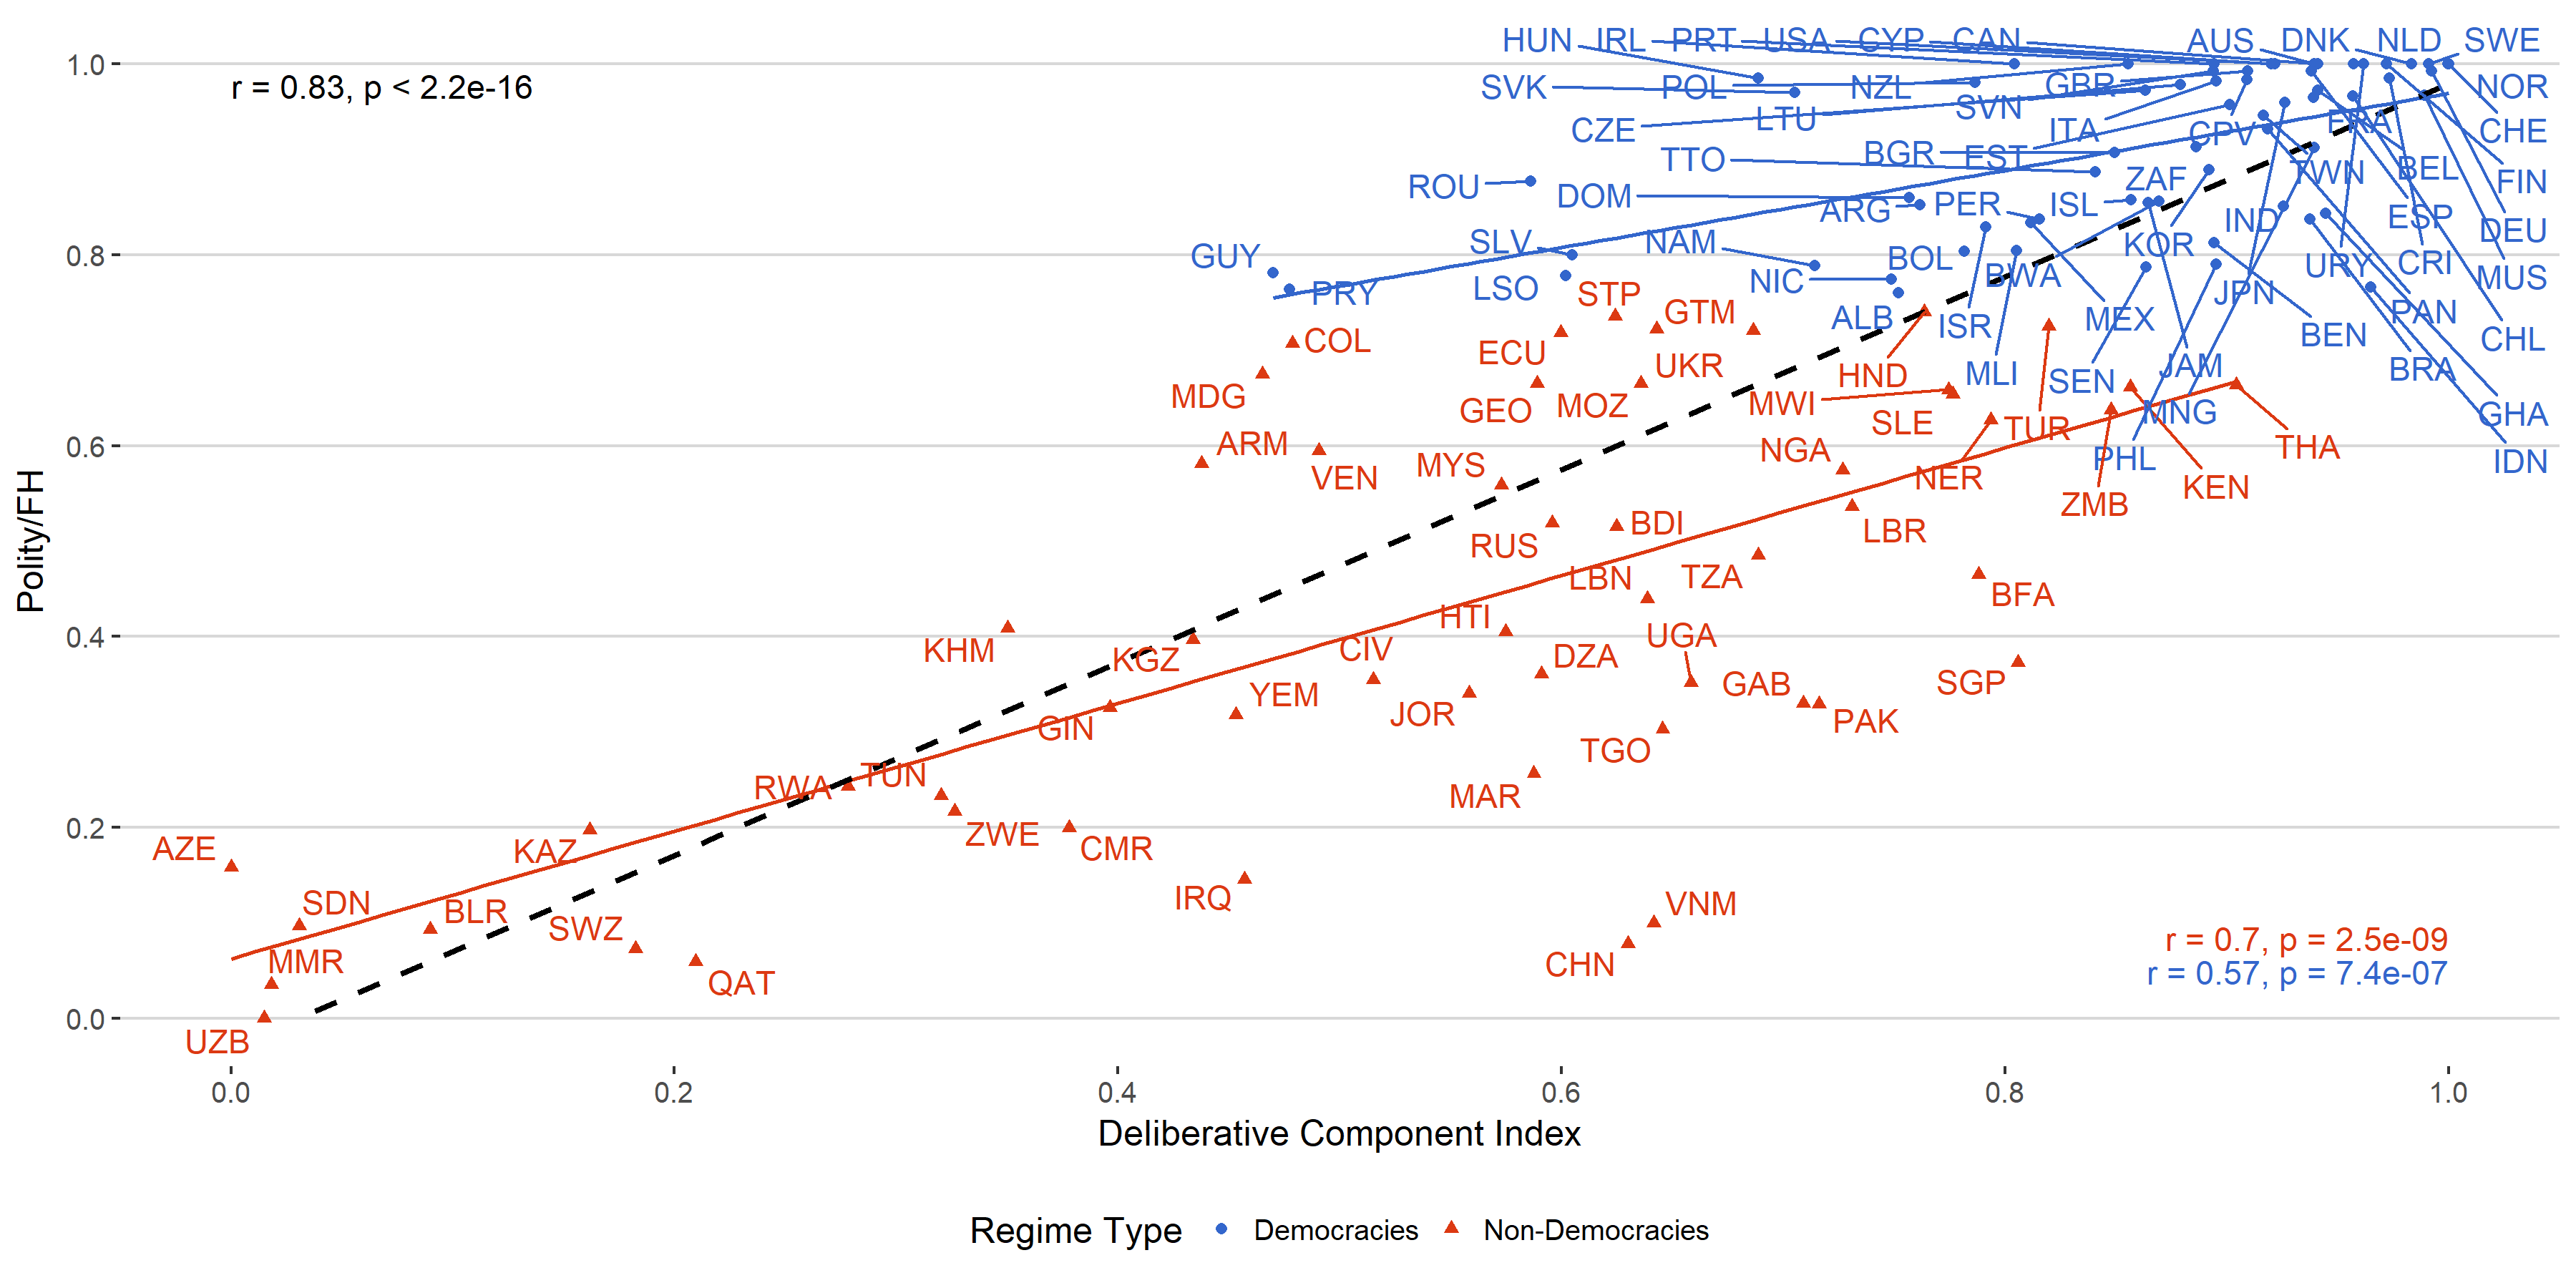
\includegraphics[width=\textwidth]{images/delib_polity.png}
    \flushright
    {\scriptsize Data Source: see Table \ref{data} in the Appendix. Own calculations.  \par}
\end{figure}

Even though deliberation and democracy are empirically strongly
connected, a closer look at the deviations seems worthwhile. Figure
\ref{chinaplot} depicts a scatterplot of the Polity/FH and DCI
variables. The blue colour resembles the democracy sample,
non-democracies are coloured red. Interestingly, the previous example of
deliberation in non-democracies, China, appears as one of the countries
which score relatively high on the DCI, especially in comparison with
the level democracy. This also applies to Vietnam and less clearly to
Singapore, both countries identified by research as non-democracies with
consultative institutions {[}cf. @jayasuriya2007more pp. 779{]}. As
China specifically was already theorized to be a case of a non-democracy
with deliberative institutions, the empirical results indicate that
there is some accuracy in the V-Dem measurement of deliberation --
despite the strong relation to democracy. There are not many deviating
cases, much less cases that deviate strongly, but if there are
differences, the results imply that they could be meaningful. Therefore,
we decide to use the DCI and its subcomponents in the analysis, with the
assumption that the diverging patterns are indeed representative of two
empirically distinct phenomena.

\begin{footnotesize}
\noindent \textbf{Control Variables}
\end{footnotesize}

Lastly, a range of control variables were added, both on the individual
and the country level, which will be described shortly (a table with all
control variables, their sources and other notes can be found in the
online appendix). On the individual level, sex, age financial security
(measured in terms of whether there is enough financial resources to
support the household), education (years of schooling and education
levels) and employment status. Other presumably important variables like
satisfaction with economy could not be included, as they are not
available across all survey projects. The macro control variables are
taken from either V-Dem, or the ``Quality of Government''-Dataset
{[}@teorell2017qog{]}. For all independent macro variables that vary
over time, the average value of the years 2000 to 2010 is calculated.
First, the already introduced Polity/FH measure serves as a control for
democracy. Furthermore, real GDP per capita in constant dollars of the
year 2000 is included (the variable is log-transformed because of severe
skewness). The third macro control variable is the population size
(natural logarithm). Further variables are the urban population ratio
and average life expectancy. Lastly, all models include design dummies
that account for the different surveys and are coded as 1 for all
respondents that were part of a specific survey project and 0 if they
were not part of it. This allows to control for possible bias between
the different survey projects.
\footnote{As it is common in cross-national studies, the analysis originally included regional dummies as controls, though the results vary strongly when including them. The varying effects within different geographical regions might need to be studied separately. As it would go beyond the scope of this study, the results including regional dummies are not reported. However, it can be said that the dataset dummies already function as regional dummies to some degree, as most of them are specific to a certain region. With that, we feel confident in reporting the results without regional dummies. Another adaptation considered, but not implemented due to the scope of the analysis, is the exclusion of specific groups of cases that could bias the results, like for example OECD or EU countries and strongly repressive regimes.}

\subsection{Possible Bias and Correction} \label{bias_section}

Given that the main variable of interest \textit{regime support}
consists of self-reported attitudes in different societies and political
systems across the world, a critical examination of the data is
appropriate. A very widespread problem within survey research is the
so-called \textit{social desirability bias}, which especially applies to
sensible survey items that concern very personal topics associated with
a social stigma {[}cf. @krumpal2013determinants{]}. Some respondents
might give responses they know to be untruthful because they either want
to comply with some strong social norms or they fear repercussions by
their social environment. Especially the fear of government repression
seems to be relevant in autocratic regimes, where expressing the wrong
opinions might lead to physical harm. That is why in such repressive
environments, respondents in surveys tend to practice
\textit{preference falsification}, where they will express
uncontroversial regime-friendly opinions in public and conceal their
real convictions {[}cf. @kuran1997private{]}. Tannenberg analyzed such
sensible survey items relating to trust in political institutions in the
context of 36 African countries and was able to show that there is
considerable bias when respondents believe that the survey is
administered by a government agency, which is especially prevalent in
more autocratic regimes {[}cf. @tannenberg2017autocratic pp. 21{]}.

There is therefore strong grounds on which it can be assumed that the
data is affected by social desirability bias, since we analyze sensible
survey items relating to regime support in environments of varying
repressiveness. In order to reveal such bias, we investigate the
relationship between our democracy measurement (Polity/FH) and regime
support, as well as a comparison of means between democracies,
anocracies and autocracies, shown in Figure \ref{comp}. Judging from the
bivariate relationship, one can notice that there seems to be a
nonlinear, rather quadratic relationship of democracy and regime
support. Very autocratic regimes score high on regime support, while
countries that are semi-democratic and democracies score noticeably
lower, although there is an uprising turn at the and of the curve,
within democratic regimes. A t-test between autocratic regimes in
regards to anocratic and democratic regimes reveals that the average
regime support is significantly higher in an autocratic context (p =
0.015 and p = 0.003), respectively, though it doesn't significantly
differ between anocracies and democracies (p = 0.24).

\begin{figure}[!htb]
    \caption{ Regime Support by Polity/FH}
    \label{comp}
    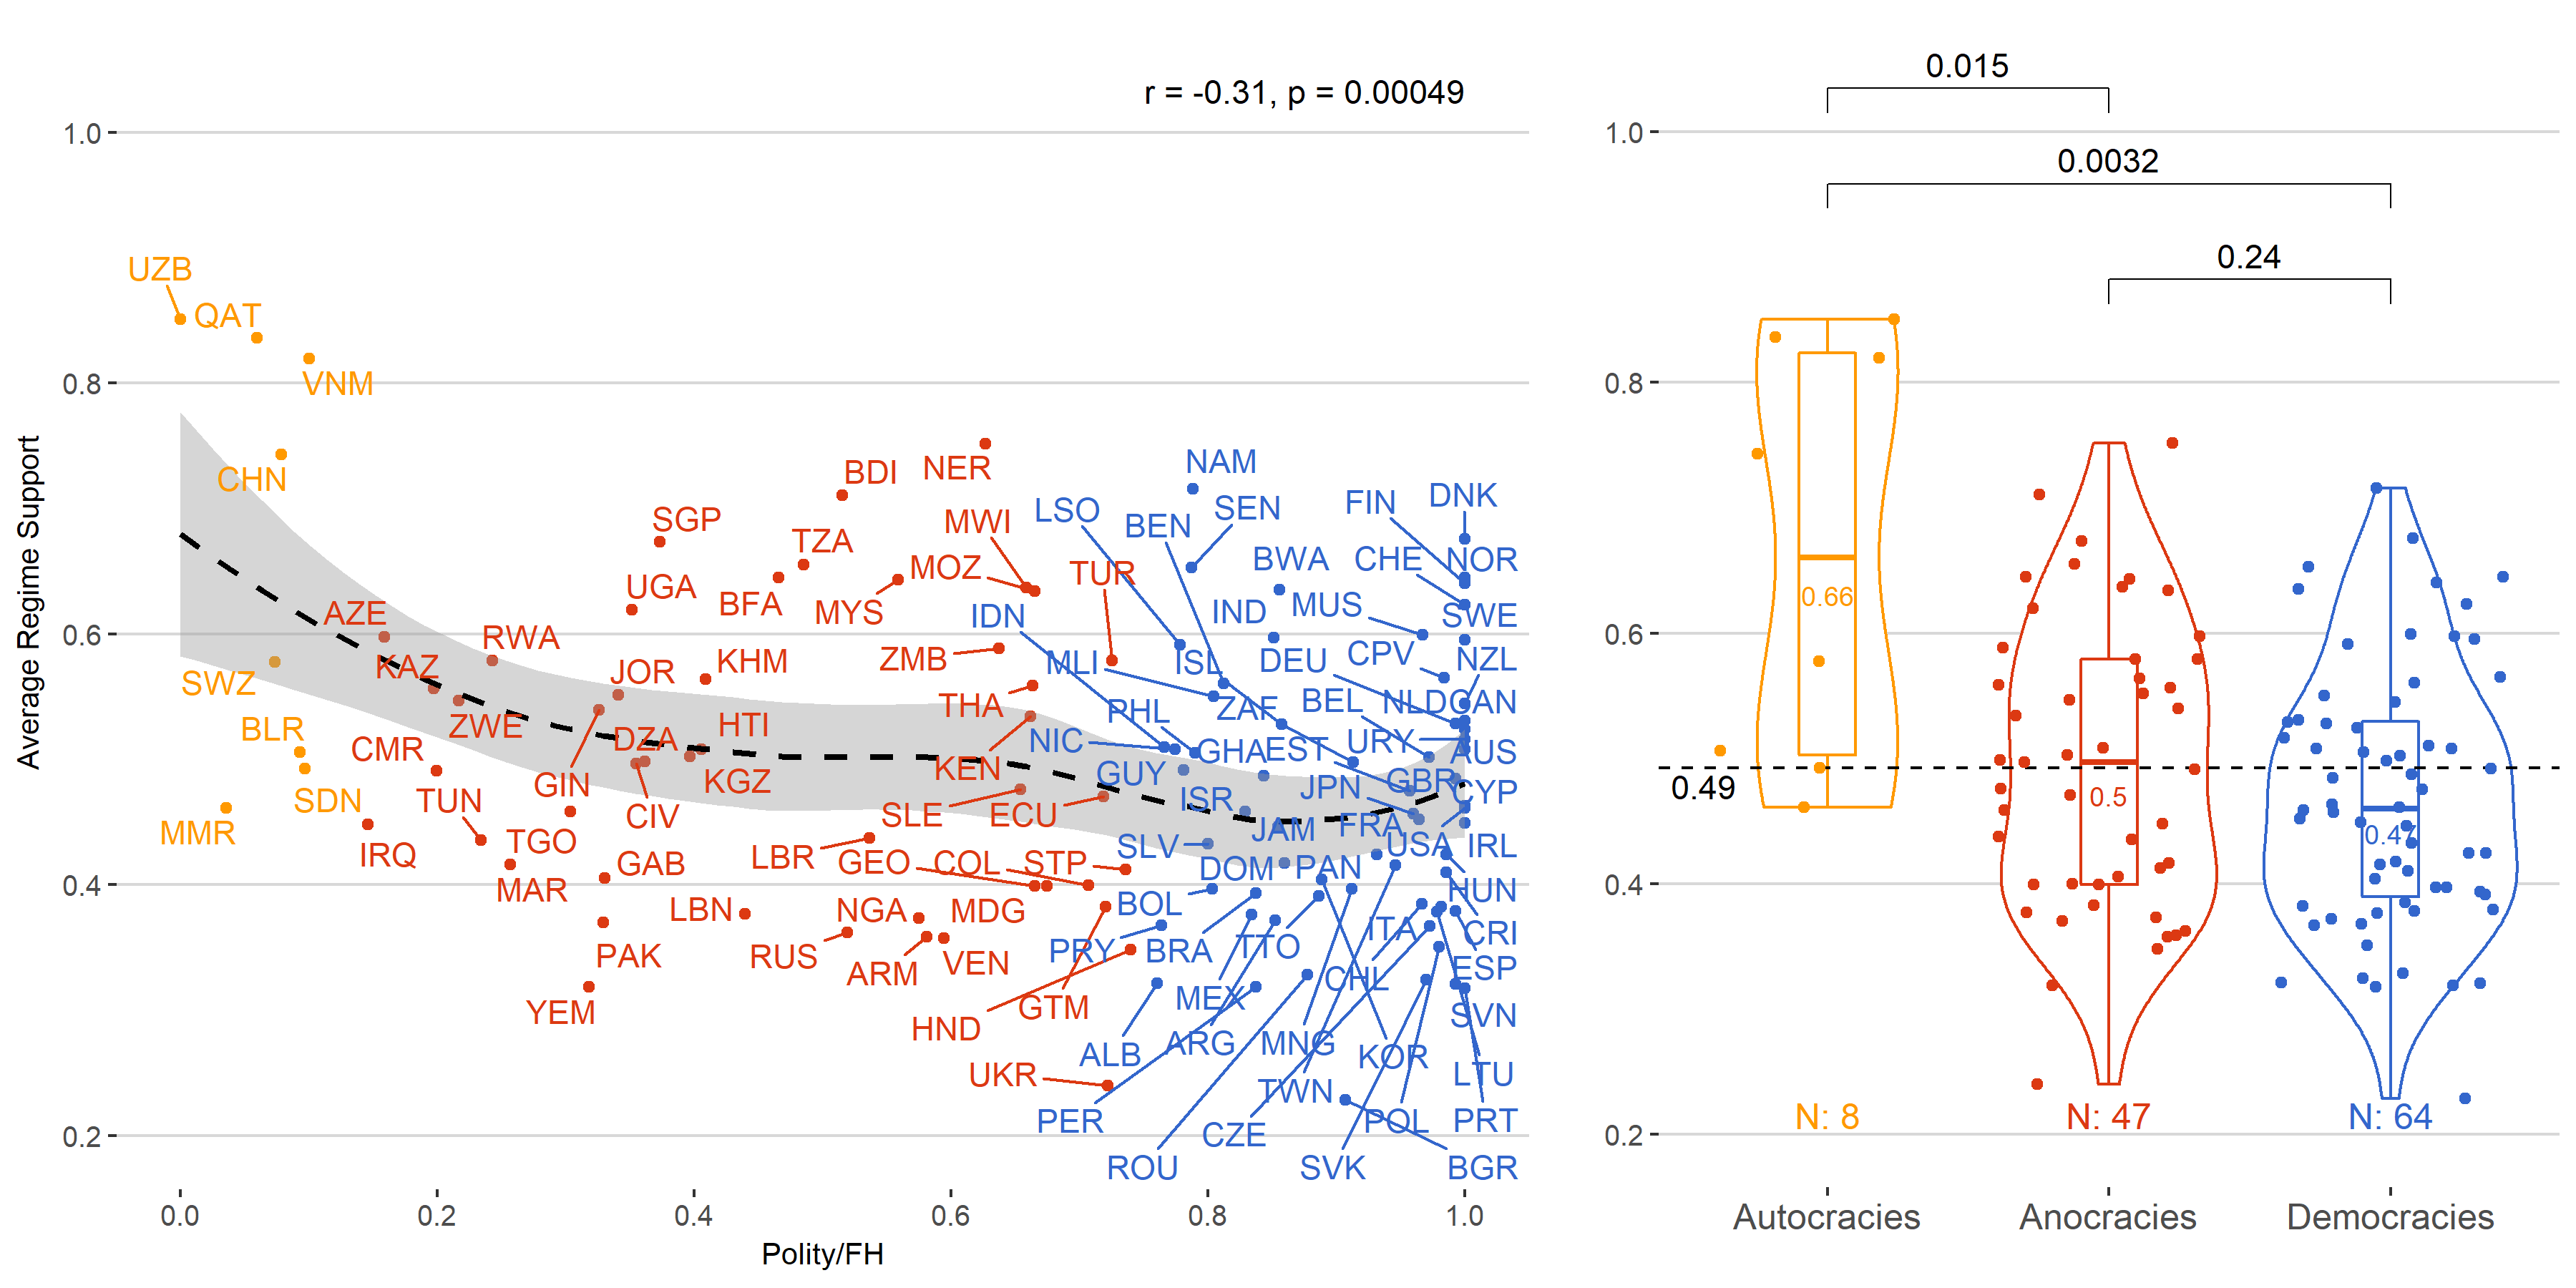
\includegraphics[width=\textwidth]{images/doubleplot.png}
    \flushright
    {\scriptsize Data Source: see Table \ref{data} in the Appendix. Own calculations.  \par}
\end{figure}

In order to investigate whether high regime support in autocracies is
due to some form of bias, a measurement of Freedom of Discussion is
introduced {[}cf. @coppedge2017v pp. 228-229{]}. Freedom of Discussion
measures ``the extent to which citizens are able to engage in private
discussions, particularly on political issues, in private homes and
public spaces {[}\ldots{}{]} without fear of harassment by other members
of the polity or the public authorities'', which has the great advantage
of not just focusing on repression of freedom of speech on behalf of the
government, but also takes into account the degree to which other
citizen impose speech prohibitions on each other. Freedom of Discussion
and regime support are positively related (see Figure \ref{comp2}),
suggesting that regime support is higher when discussion about political
issues is less free. This might imply that revealing low support of the
regime is socially undesirable and politically inconvenient in such
societies and therefore citizen tend to falsify their preferences and
express higher levels of regime support to avoid negative repercussions.

\begin{figure}[!htb]
    \caption{Regime Support by Freedom of Discussion}
        \label{comp2}
    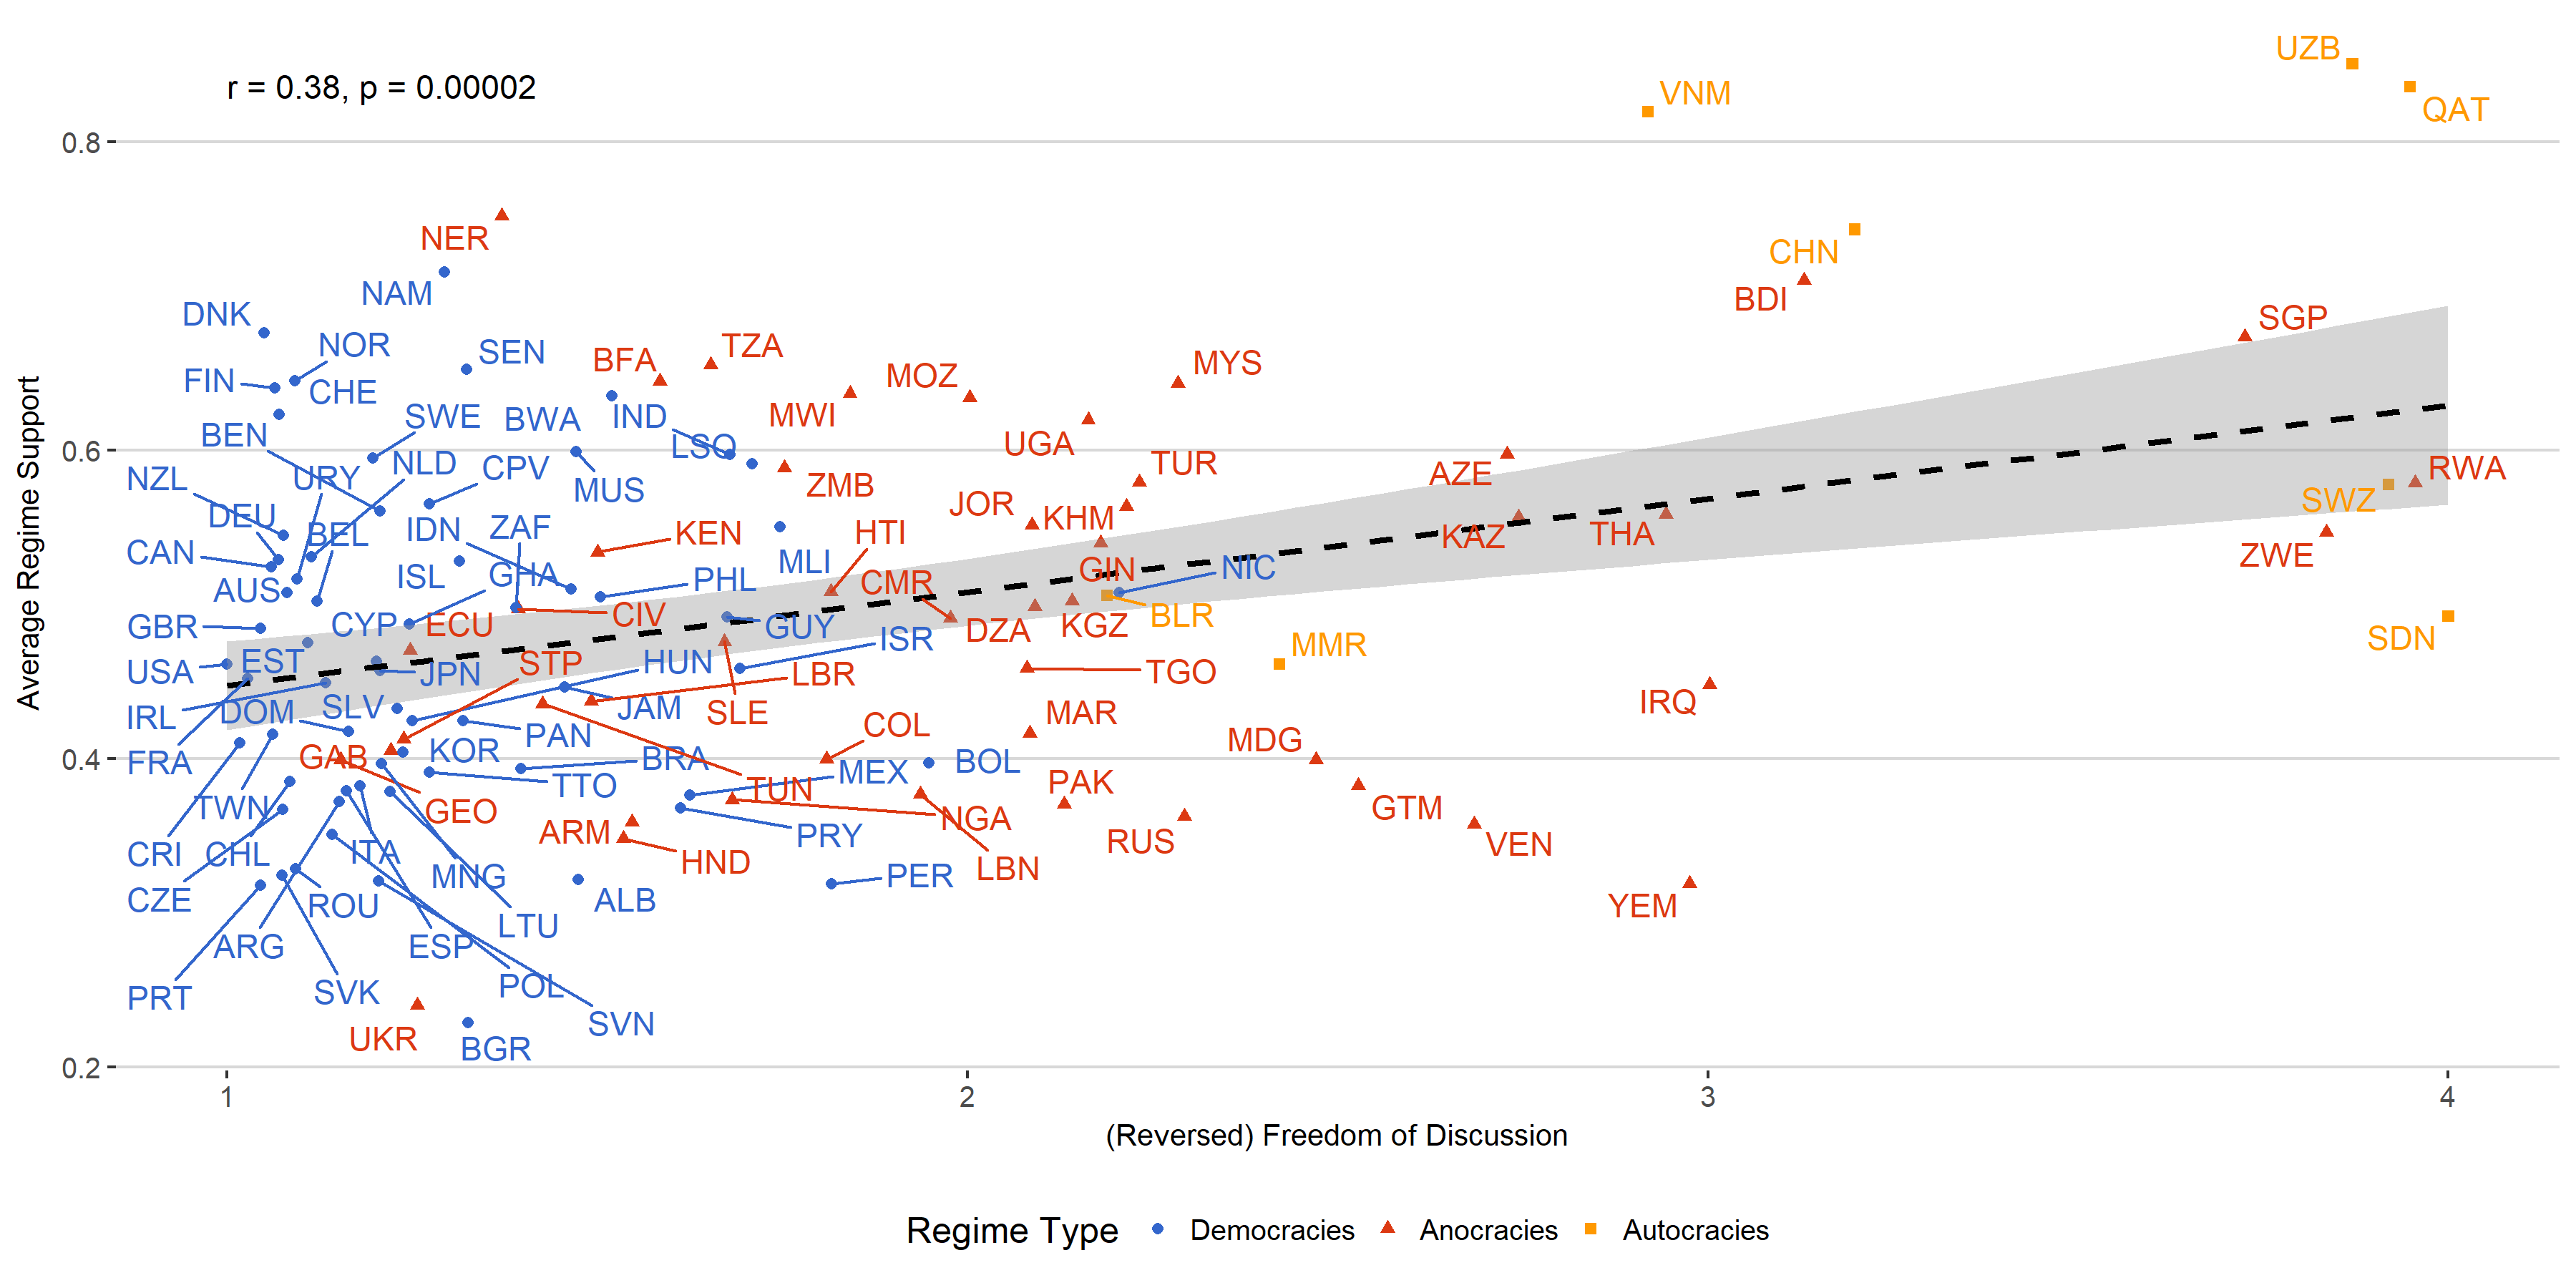
\includegraphics[width=\textwidth]{images/regimesupport_fod.png}
    \flushright
{\scriptsize Data Source: see Table \ref{data} in the Appendix. Own calculations.  \par}
\end{figure}

This possible bias in the data poses a serious problem for the analysis.
What is to be done to remedy the revealed problematic? Two such
approaches might be suitable: 1.) exclude the countries that are most
likely to be biased or 2.) design a weight that accounts for the
possible bias. The first approach may limit the validity of the results
because it is associated with a loss of information, and also
systematically leaves out a certain group of countries. A designed
weight seems the more appropriate adaptation, as Tannenberg recommends:
``one avenue forward would be to construct reliability weights to enable
the researcher to account for the biases in the analysis''
{[}@tannenberg2017autocratic pp. 21{]}. Unfortunately, variables
indicating whether respondents believed the surveyors to be government
representatives or other possible weighting variables are not available
for all surveys used in this analysis, therefore a weight on the
country-level might be an alternative. We therefore use the Freedom of
Discussion measurement to weigh regime support, which is already proven
to be positively associated. Given that the proposed weight is highly
experimental in nature, two bias boundaries will be introduced: a lower
and a higher bound, whereby regime support in societies with somewhat
and weakly respected Freedom of Discussion will be penalized with 10\%
and 15\% (low bias) or 20\% and 25\% (high bias), respectively. Table
\ref{weight} shows a summary for all weighted country cases, which only
applies to anocratic and autocratic regimes.

\begin{table}[!htb]
    \centering
    \caption{Weighting of Regime Support}
    \label{weight}
    \resizebox{\textwidth}{!}{%
        \begin{tabular}{@{}lcccl@{}}
            \toprule
            \textbf{Country}    & \multicolumn{1}{c}{\begin{tabular}[c]{@{}c@{}}\textbf{Regime Support} \\ \textit{Original}\end{tabular}} & \multicolumn{1}{c}{\begin{tabular}[c]{@{}c@{}}\textbf{Regime Support}\\ \textit{Low Bias (10 - 15\%)}\end{tabular}} & \multicolumn{1}{c}{\begin{tabular}[c]{@{}c@{}}\textbf{Regime Support} \\ \textit{High Bias (20 - 25\%)}\end{tabular}} & \multicolumn{1}{c}{\begin{tabular}[c]{@{}c@{}}\textbf{Freedom of Discussion}\\ \textit{(FoD)}\end{tabular}} \\ \midrule
            Qatar      & 85.68                                                                                  & 72.83                                                                                             & 64.26                                                                                               & \textit{Weakly Respected}                          \\
            Uzbekistan & 82.97                                                                                  & 70.53                                                                                             & 62.23                                                                                               & \textit{Weakly Respected}                          \\
            Singapore  & 68.06                                                                                  & 57.85                                                                                             & 51.04                                                                                               & \textit{Weakly Respected}                          \\
            Kuwait     & 66.50                                                                                  & 56.52                                                                                             & 49.87                                                                                               & \textit{Weakly Respected}                          \\
            Swaziland  & 59.07                                                                                  & 50.21                                                                                             & 44.30                                                                                               & \textit{Weakly Respected}                          \\
            Rwanda     & 57.38                                                                                  & 48.77                                                                                             & 43.03                                                                                               & \textit{Weakly Respected}                          \\
            Zimbabwe   & 55.08                                                                                  & 46.82                                                                                             & 41.31                                                                                               & \textit{Weakly Respected}                          \\
            Vietnam    & 79.98                                                                                  & 71.98                                                                                             & 63.99                                                                                               & \textit{Somewhat Respected}                        \\
            China      & 71.28                                                                                  & 64.15                                                                                             & 57.02                                                                                               & \textit{Somewhat Respected}                        \\
            Burundi    & 68.80                                                                                  & 61.92                                                                                             & 55.04                                                                                               & \textit{Somewhat Respected}                        \\
            Thailand   & 58.17                                                                                  & 52.36                                                                                             & 46.54                                                                                               & \textit{Somewhat Respected}                        \\
            Azerbaijan & 56.78                                                                                  & 51.10                                                                                             & 45.43                                                                                               & \textit{Somewhat Respected}                        \\
            Kazakhstan & 52.24                                                                                  & 47.02                                                                                             & 41.79                                                                                               & \textit{Somewhat Respected}                        \\
            Iraq       & 49.90                                                                                  & 44.91                                                                                             & 39.92                                                                                               & \textit{Somewhat Respected}                        \\
            Guatemala  & 38.52                                                                                  & 34.66                                                                                             & 30.81                                                                                               & \textit{Somewhat Respected}                        \\
            Madagascar & 36.67                                                                                  & 33.00                                                                                             & 29.34                                                                                               & \textit{Somewhat Respected}                        \\
            Venezuela  & 34.76                                                                                  & 31.29                                                                                             & 27.81                                                                                               & \textit{Somewhat Respected}                        \\ \toprule
            \textit{Correlation - FoD}  & \textit{0.38}                                                                                  & \textit{0.20}                                                                                            & \textit{0.04}                                                                                               & -                        \\ \bottomrule         \\[-1em]
            \multicolumn{5}{l}{%
                \begin{minipage}{20cm}%
                    \flushright
                    \scriptsize Pearson's r reported. Data weighted to same sample size (=1000). Data Source: see Table \ref{data} in the Appendix. Own calculations.%
                \end{minipage}%
            }
        \end{tabular}
    }
\end{table}

One caveat comes with this approach: as it stands, Freedom of Discussion
is positively associated with democracy (r = 0.78 for the whole sample,
and r = 0.59 within non-democracies) and also associated with increased
deliberative levels (r = 0.65 with DCI for the complete sample, and r =
0.43 for the non-democracy subsample). Thereby, weighting regime support
with Freedom of Discussion inherently makes the dependent variable more
similar to the independent variables. However, the usage of the weight
can be well justified on theoretical grounds and it is thereby assumed
that this adaptation improves the validity of measured regime support.
Nevertheless, this step has to be critically evaluated, as we might
over- or underestimate the bias severely. Therefore, models with
unweighted regime support are always reported as well.

\subsection{Descriptives} \label{descr_section}

This section will examine some of the descriptive statistics and
bivariate correlations, focusing on the relationship between
deliberation and regime support, but also including levels of democracy
to account for the necessity to separate democracy and deliberation. As
a first overview, the left-hand side of Figure \ref{map2} depicts a map
with levels of regime support across the world. Grey coloring indicates
that data for the country wasn't available. First, it comes to attention
that there is no clear regional pattern of regime support in our sample,
although some general trends can be observed. Firstly, Northern Europe
stands out with higher levels of support, with much of Western and
especially Southern and Eastern Europe having lower support. Then,
available cases in Southern and Eastern Africa score high mostly,
whereas Western Africa shows a rather mixed pattern. For the MENA
countries, it becomes visible that they are highly underrepresented.
Turning the attention to Asia, the relatively high average regime
support, especially in parts of Eastern and South-Eastern Asia stand
out. Across Central and South America, there is no country with above
medium levels, indicating rather low aggregate levels of regime support
within the broader region. The right-hand side of Figure \ref{map2}
shows a world map indicating the DCI score (normalized to range from
0-1) across the countries of our sample. Notably, the distribution of
the DCI is rather skewed, which leaves us with few cases having low
scores. The regional patterns for the DCI differ from the ones of regime
support. First, Northern as well as Western and Southern Europe are all
placed within the higher quintiles. Concerning the Americas, a mix of
medium to high levels of deliberation can be found. The pattern for
African countries is also mixed, with more countries scoring lower on
the DCI. In Asia, the pattern is rather ambiguous as well, though
especially South-Eastern Asia stands out with comparably higher scores
on the DCI.

\begin{figure}[!t]
    \caption{Regime Support \& Deliberation Across the World}
    \label{map2}
    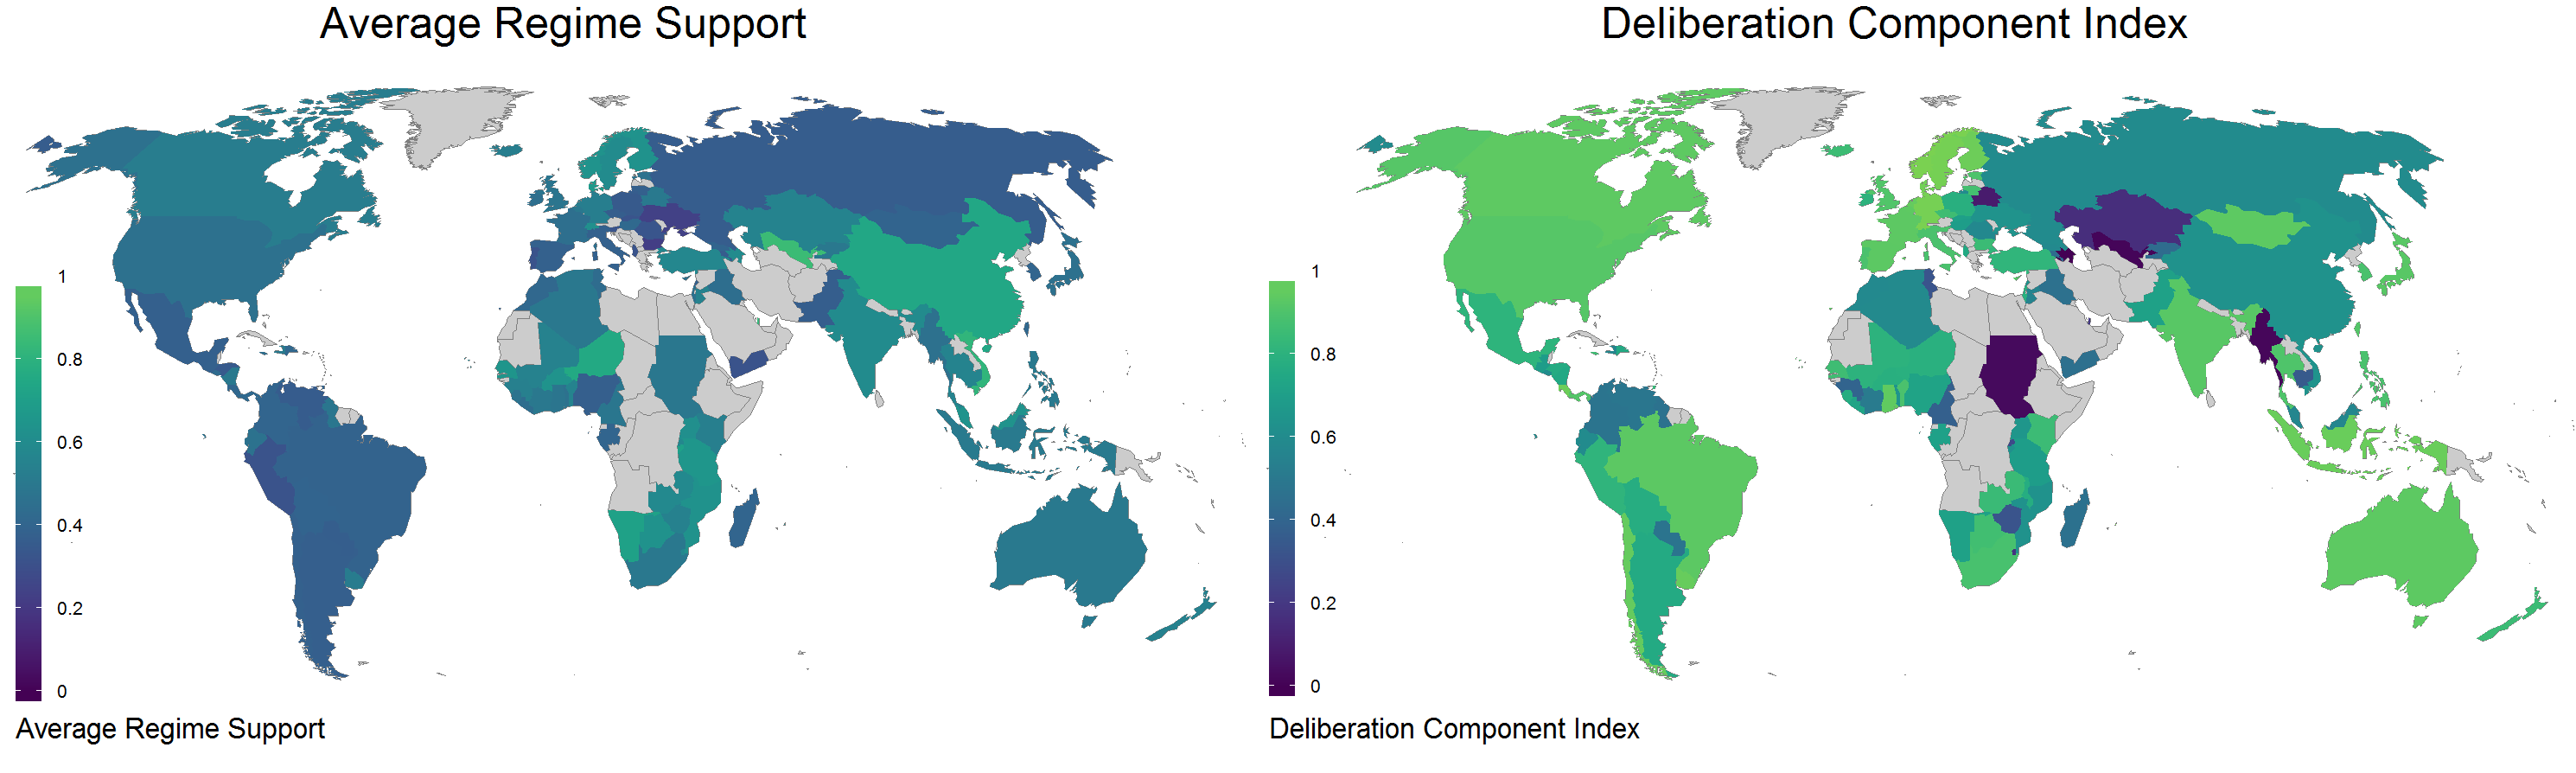
\includegraphics[width=\textwidth]{images/map2.png}
    \flushright
{\tiny Data Source: see Table \ref{data} in the Appendix. Data weighted to same sample size (=1000).  Own calculations.  \par}
\end{figure}

Figure \ref{sixs} shows scatterplots that visualize the distribution of
average regime support (all three variants) per country over levels of
deliberation (the DCI and its components, respectively). The dashed line
shows the overall correlation. The coloring of the cases is yellow for
autocracies, red for anocracies and and blue for democracies. In the
first column, the correlations are shown for the unweighted regime
support, the second and third column depict the results for the low bias
and high bias variables respectively (the correlations within
democracies don't change, as they aren't affected by the weighting).
When only observing overall correlations, it comes to attention that all
deliberation indicators have almost no observable effect sizes, with a
stronger tendency to a negative relationship for the unweighted regime
support. Regarding the weighted independent variables, especially the
high boundary one, the correlations become weakly positive, although the
effect sizes are rather small. Interestingly, when grouped into regime
type categories, there is a consistent pattern that shows mostly
stronger or sometimes equal positive correlations within the groups
compared to the overall relationship. This counts not as much for
anocracies, for which correlations are sometimes less strong and
generally more in line with the overall sample. In contrast to the
relatively small bivariate correlation within the full dataset, the
deliberation indicators seem to be consistently positively related to
regime support within groups of similar levels of democracy. In sum, the
findings of the bivariate correlations indicate that deliberation and
regime support are related first and foremost in democracies, and also
in autocratic states, although the number of cases for this group is
relatively small. For anocracies, the results are not as clear, although
they mostly point into the same direction. As the results discussed here
are not controlled for other variables, this should be seen as a first
indication rather than an explicit finding.

\begin{figure}
        \caption{Bivariate Relationships between Deliberation Indicators and Regime Support}
        \label{sixs}
    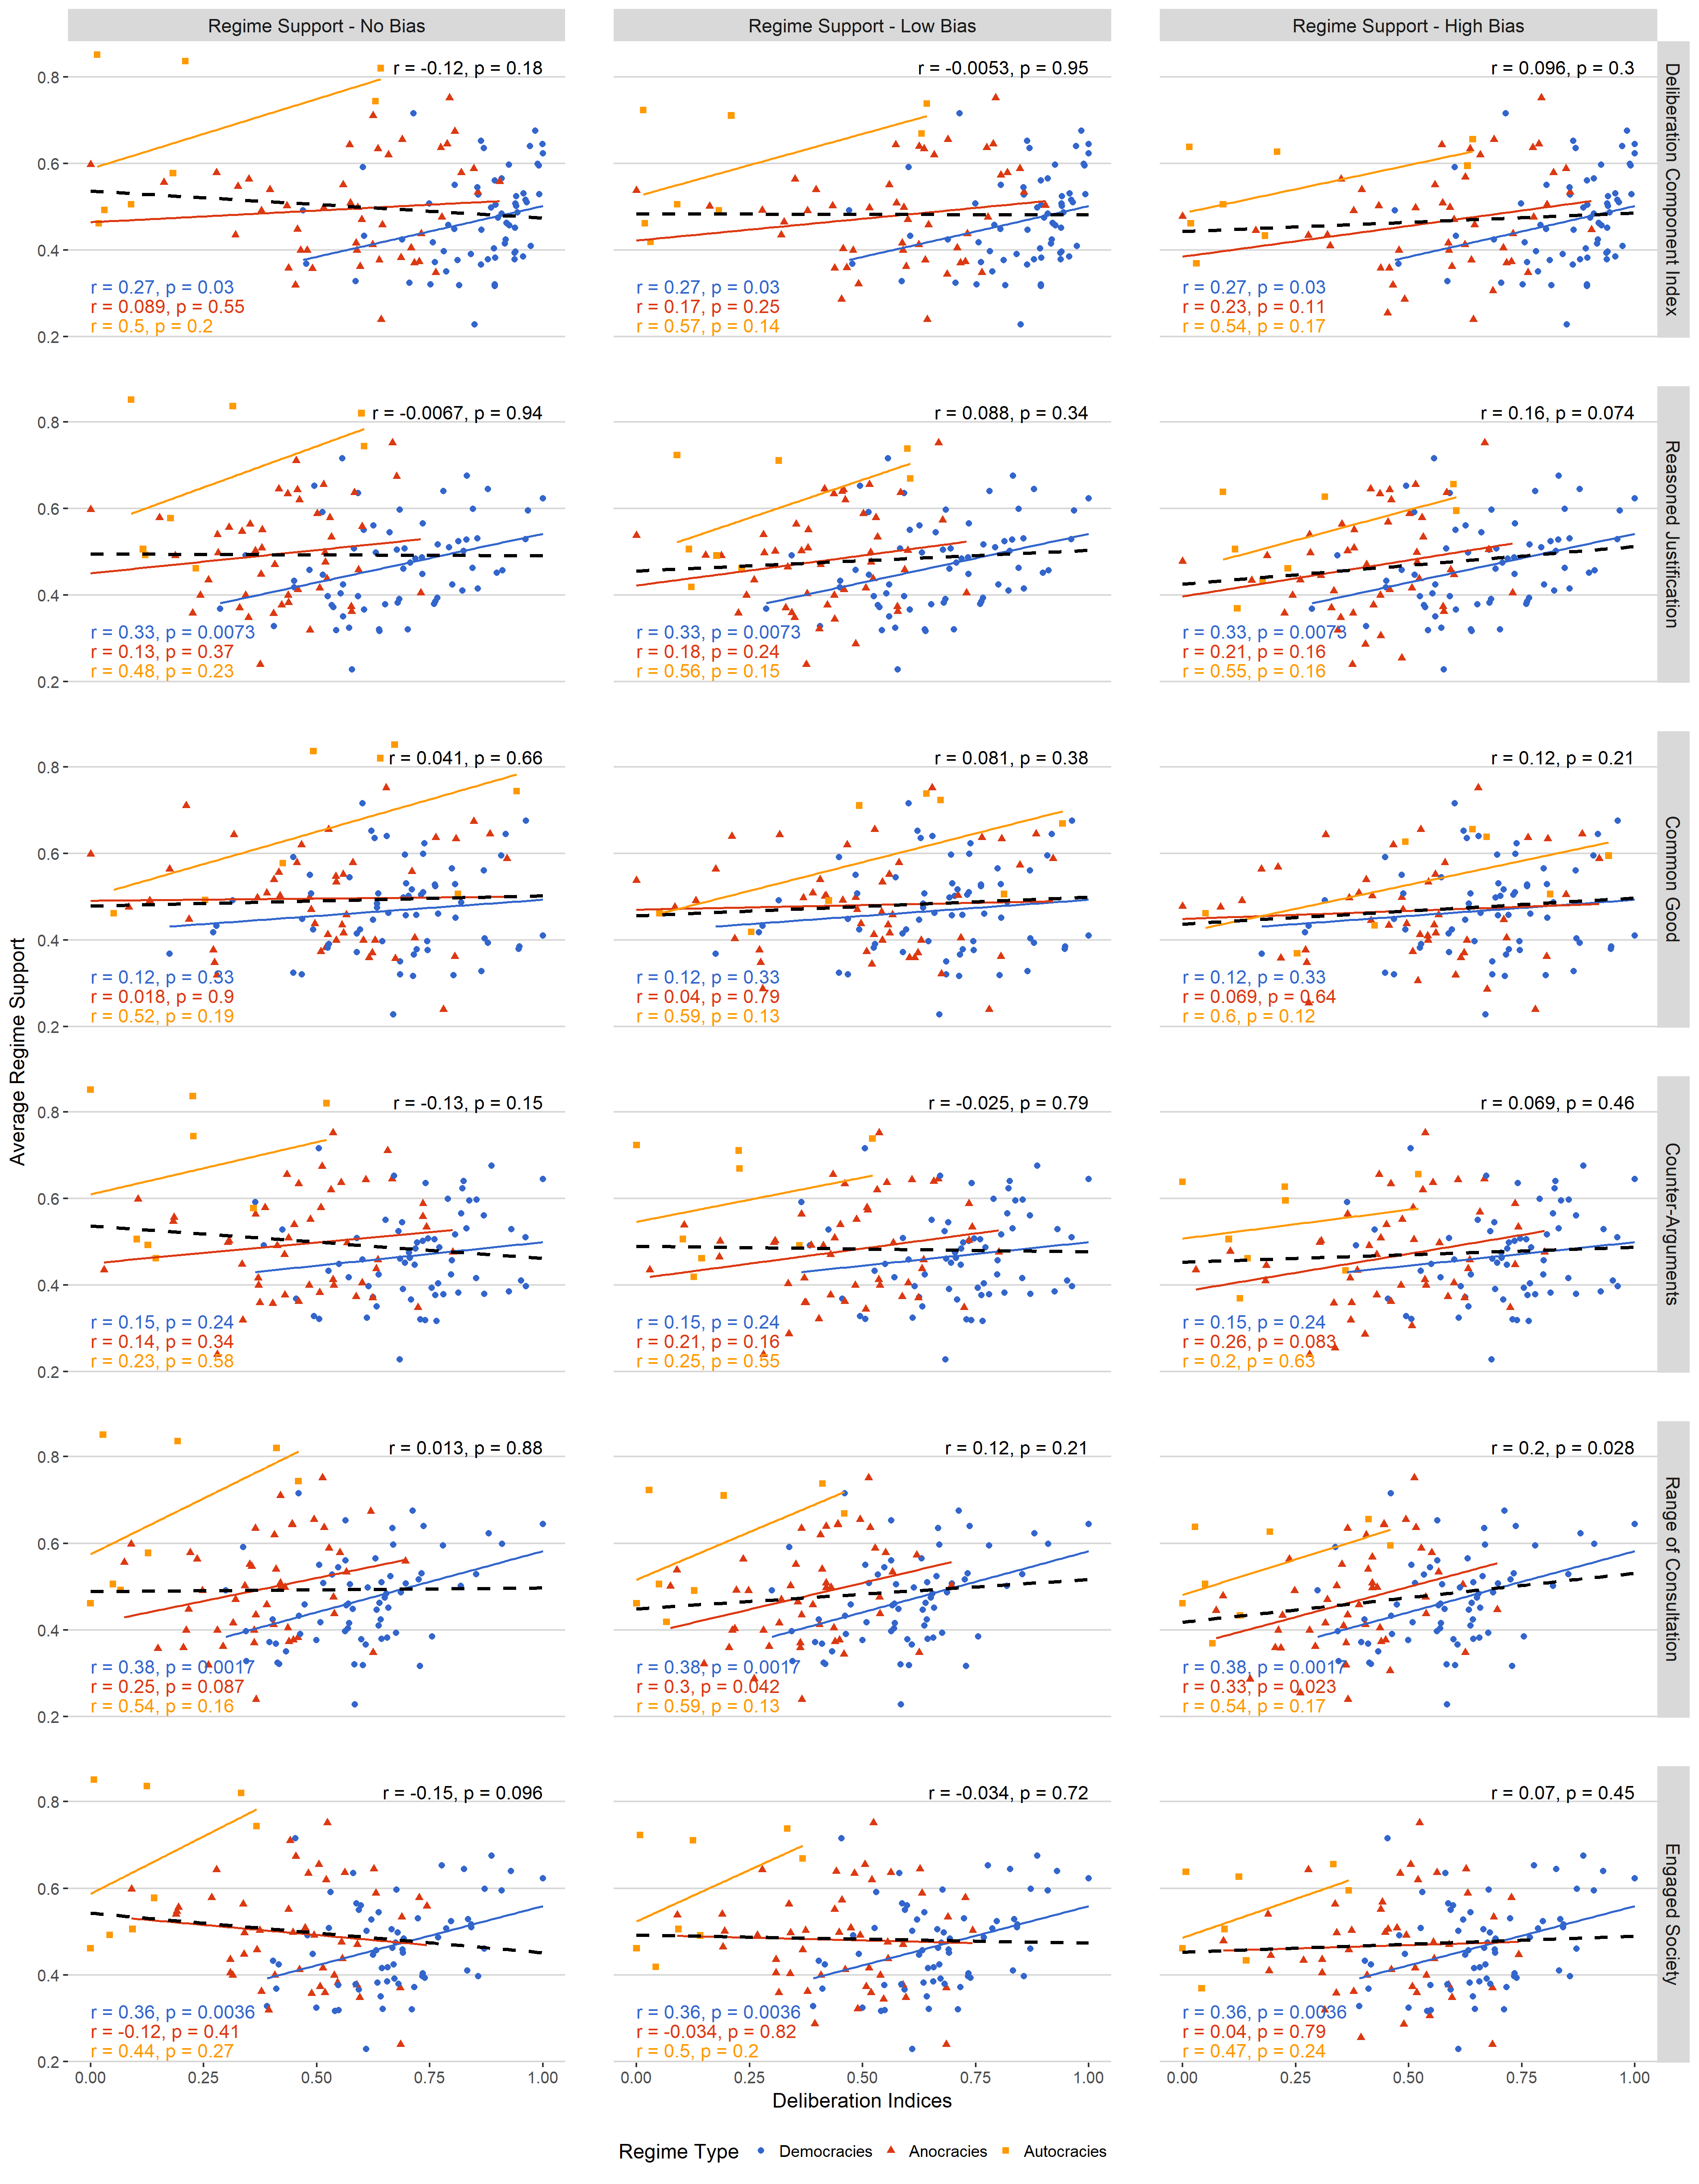
\includegraphics[width=\textwidth]{images/megaplot.png}
        \flushright
        {\scriptsize Data Source: see Table \ref{data} in the Appendix. Data weighted to same sample size (=1000). Persons’s r is reported. Own calculations.  \par}
\end{figure}

In sum, the findings of the bivariate correlations indicate that
deliberation and regime support are related first and foremost in
democracies. This could imply that deliberation is - in fact - a
predominantly democratic concept that only works within the freedoms
that come along with democratic regimes. As the results discussed here
are not controlled for other variables, this should be seen as a first
indication rather than an explicit finding.

\subsection{Multilevel Regression Analysis} \label{multilevel_section}

\begin{Shaded}
\begin{Highlighting}[]
\KeywordTok{load}\NormalTok{(}\StringTok{"data/estimate_data.Rdata"}\NormalTok{)}

\NormalTok{cite_b <-}\StringTok{ }\ControlFlowTok{function}\NormalTok{(model, term) \{}
\NormalTok{  estimates_data }\OperatorTok\StringTok{ }
\StringTok{  }\KeywordTok{filter}\NormalTok{(model_cite }\OperatorTok{==}\StringTok{ }\OperatorTok{!!}\NormalTok{model) }\OperatorTok\StringTok{ }
\StringTok{  }\KeywordTok{filter}\NormalTok{(term_cite }\OperatorTok{==}\StringTok{ }\OperatorTok{!!}\NormalTok{term) }\OperatorTok\StringTok{ }
\StringTok{  }\KeywordTok{mutate}\NormalTok{(}\DataTypeTok{estimate =} \KeywordTok{sprintf}\NormalTok{(}\StringTok{'%.2f'}\NormalTok{, estimate, }\DecValTok{2}\NormalTok{)) }\OperatorTok\StringTok{ }
\StringTok{  }\KeywordTok{select}\NormalTok{(estimate) }\OperatorTok\StringTok{ }
\StringTok{  }\KeywordTok{as.character}\NormalTok{()}
\NormalTok{\}}

\CommentTok{# estimates_data}
\CommentTok{# }
\CommentTok{# cite_b("B2.1", "reason10")}
\CommentTok{# cite_b("E1.5", "polity_demdummy")}
\end{Highlighting}
\end{Shaded}

A range of multilevel models are then estimated in order to test the
assumptions derived in the theoretical part.\footnote{Given that the
  dataset in this paper combines individual level data with country
  level data, a multilevel analysis is needed to account for
  hierarchical data structure, which will model a unique intercept for
  each country {[}cf. @gelman2006data pp. 237{]}. This becomes
  necessary, because standard linear regression only produces accurate
  estimations of standard errors if the data points are independent of
  each other, which is not the case in our dataset. Furthermore, since
  the main independent variable is located on the country-level, it
  allows us to control its influence for individual-level control
  variables. We follow a recommendation by Enders and Torighi to use
  grand-mean centered predictors, because a multilevel analysis with the
  focus on the influence of a level 2 predictor can then be controlled
  by the individual level variables (as it is our intent) {[}cf.
  @enders2007centering pp. 128 - 129{]}.} First, in order to assess
whether multilevel modeling is warranted, a null model for each
dependent variable is estimated (weighted and unweighted) with a
random-intercept and no predictors {[}cf. @hox2010multilevel pp. 300{]}.
The intraclass correlations (ICCs) for the null models show that indeed
44.97\% (unweighted), 41.70\% (low boundary weight) and 40.97\% (high
boundary weight) of the variance of regime support is bound on the
country-level. The results strongly indicate that a multilevel analysis
is appropriate. Given the expected high levels of multicollinearity, the
influence of DCI and its subcomponents on regime support is tested
separately for the Polity/FH variable, in order to control for possible
distortions caused by the strong overlap between the two variables. In
the interest of accounting for the slight quadratic effect in the
relationship between democracy and regime support in the complete
sample, the Polity/FH variable will be split into three dummies,
Autocracy, Anocracy and Democracy, as recommended by
@tabachnick2013using {[}pp. 43-44{]}. Moreover, in order to avoid issues
of multicollinearity, the sample is further divided into democracies
(Polity/FH \(\ge\) 6) and non-democracies (Polity/FH \(<\) 6). In these
subsamples, the continuous Polity/FH variable can be used again, because
the quadratic relationship only appears in the full sample. These
divisions of the sample, in addition to estimating all models for three
separate dependent regime support variables (no bias, low bias, high
bias), six separate independent deliberation variables, as well as with
and without Polity/FH, leaves us with 84 multilevel models to be
estimated. In addition, we estimate seven models with Polity/FH only and
none of the deliberation indicators, for the purpose of comparison,
which adds up to a total of 91 estimated models. Given the exploratory
nature of the analysis and the many problems with expected
multicollinearity and quadratic effects, the estimation of so many
models seems justified as this allows us to test for robustness of the
findings. To facilitate an intuitive communication of the results, we
will only visualize the relevant effects in the main text and report the
detailed results in tables in the online
appendix.\textbackslash{}footnote\{Since multicollinearity was expected
for many of the estimated models, it should be noted right at the
beginning that none of the 91 estimated regression models in the
analysis showed problematic VIF-values for any of the included variables
(VIF \(<\) 5 in all estimated models). Furthermore, regression
diagnostics for one of the full models involving the DCI and all control
variables has been conducted and no major violation of statistical
assumption are revealed (results are reported in the online appendix).

Figure \ref{reg1} summarizes the unstandardized regression coefficients,
the bold lines indicating a 95\% confidence interval, the thin lines a
90\% interval for the effects of DCI and its components (estimated
separately, not included in one model) on three different dependent
variables: regime support with no weighting (colored in blue),
weightings applied with low (red) and high boundaries (yellow),
respectively (the full report of all 36 estimated models can be found in
the online appendix). The Graph on the left side of the Figure depicts
the effects are controlled for variables on the individual level (Age,
Sex, Education, Financial Security, Employment) along with country level
variables (logged GDP, logged Population, Life Expectancy, Urban
Population Ratio ).When investigating the results for, the findings are
mixed. For the unweighted dependent variable, three indicators have weak
negative effects on regime support, two positive and one is not
discernible at all. A continuous pattern catches one's attention: the
weighting of the dependent variable causes the coefficients for all
deliberation indicators to shift towards positive effects. For the high
boundary weighting, none of the coefficients is negative anymore, with
effect sizes varying from 0.05 to
0.14.\footnote{The shift towards more positive effects is (maybe just partly) an inherent consequence of the weighting, as discussed before. Of course, the unweighted results have the problem of assumably being (more) biased, and therefore estimates should be interpreted with caution.}
It has to be noted that the models reported here do not separate the
effects of democracy and deliberation, which suggests that the effects
might be strongly interwoven, given the high correlation between both
measures.

\begin{landscape}
    \begin{figure}
        \caption{Complete Sample: Models A1.1 to F1.6}
        \label{reg1}
        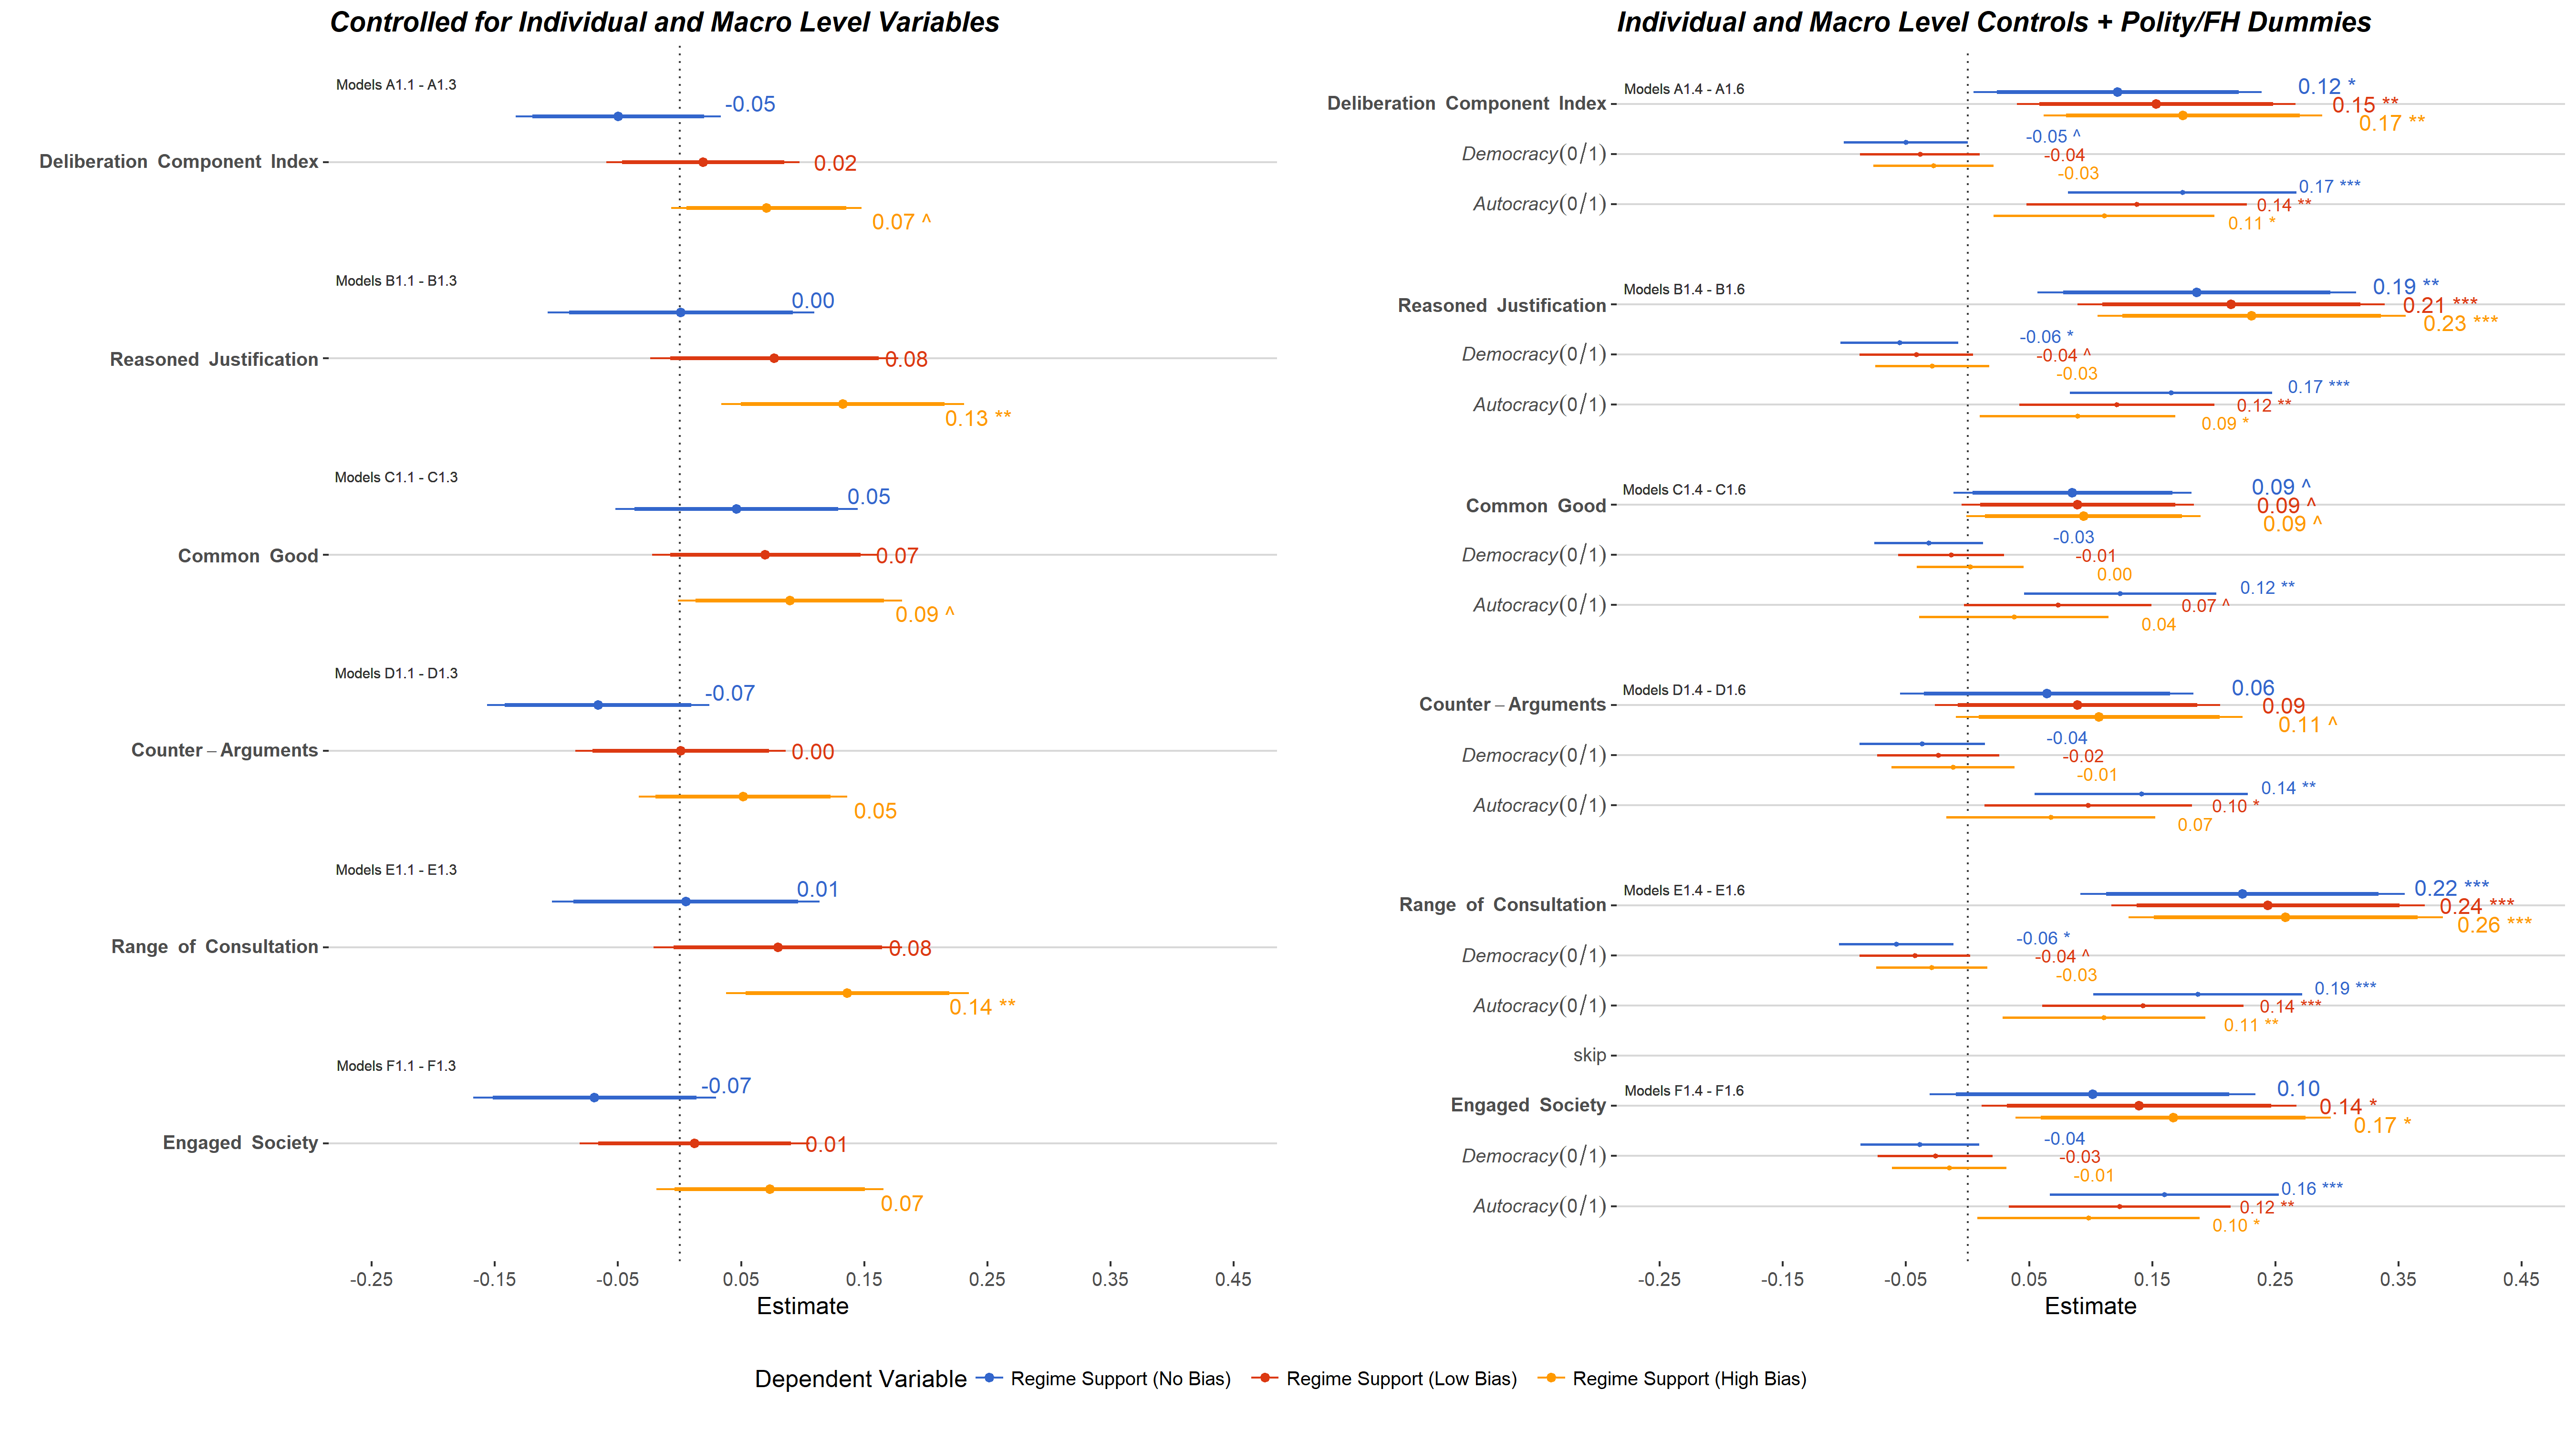
\includegraphics[width=690pt,height=530pt]{images/coefplot.png}
        \flushright
        {\scriptsize $^{***}p<0.001$, $^{**}p<0.01$, $^*p<0.05$, $^{\dagger}p<0.1$. Standardized regression coefficients and 90\% confidence intervals are reported. Reference category for Polity/FH dummies is Anocracy. For the full models see Appendix Table \ref{mod1} and \ref{mod2}. Data weighted to same sample size (=1000). Data Source: see Table \ref{data} in the Appendix. Own calculations  \par}
    \end{figure}
\end{landscape}

The second column of Figure \ref{reg1} depicts the results for models
that include individual- and country-level variables including dummies
for Polity/FH (Autocracies and Democracies, with Anocracies as reference
category). As discussed before, we refrain from using a continuous
variable because the specification of a quadratic term for Polity/FH, to
capture the nonlinear effect more adequately, would increase already
existing problems of multicollinearity. For the interpretation of the
reported results, it has therefore to be noted that the effect of
democracy is controlled for in a restricted manner. Including the
Polity/FH dummies has a striking impact on the coefficients of all six
deliberation indicators. For all of the independent variables, the
effects shift towards (more) positive effects of the respective
deliberation indicators, although the effect sizes stay rather weak. In
general, the coefficients of the Polity/FH dummies show that regime
support is higher in autocracies than in anocracies and in turn lower in
democracies than in anocracies. It has to be noted, that this applies
for the high boundary dependent variable as well. This could mean, that
our weighting is not accurate or strong enough. One the other hand, the
possibility that autocracies and to a lesser degree anocracies actually
do enjoy more or at least equal support from their citizens than
democracies has to be considered. For example, citizens in democracies
could be more ``assertive'' than ``allegiant'' {[}cf.
@welzel2015assertive{]}. In light of the current ``disconnect'' many
democracies are said to experience {[}cf. @foa2016democratic{]}, the
assumption that regime support is not higher in democracies does not
seem completely far-fetched. It has to be noted, though, that the
effects of both dummies are notably weaker when only the dummies and
control variables, but none of the deliberation indicators are included
(Models P.1.1 to P1.3, see online appendix).

Lastly, we compare the estimated models reported on the left and right
side of Figure \ref{reg1}, with the help of the deviance (-2 times the
log-likelihood). The models are compared with the respective Polity/FH
only models as well. The purpose of this comparison is to evaluate
whether the deliberation indicators contribute to a better model fit,
especially in comparison with models including only the Polity/FH
dummies (see online appendix). The models A2.4 to F2.6 (with Polity/FH
dummies and the deliberation indicators included) fit consistently
better than the models A1.1 to F1.3 (including only the deliberation
indicators), with some minor exceptions. In comparison to the models
including only the dummy variables (P1.1 to P1.3), the models also
including the DCI , Reasoned Justification, Common Good and Range of
Consultation fit consistently better than their respective counterparts.
For Counter-Arguments and Engaged society, a better fit can only be
observed for the High and Low Bias dependent variables.

In conclusion, for the assumption that deliberation has a positive
effect on regime support, the findings are mixed. In models not
controlling for Polity/FH dummies and using unweighted regime support,
there is no evidence for the proposed relationship. Then again, when
assuming that the data is biased and that the applied weightings
actually remedy the bias, and when including dummies for democracy and
democracy, one could conclude that deliberation actually has positive
effects. As the assumption of the accuracy of the applied weighting
isn't tested, and the effects when including the Polity/FH dummies is
suspicious due to expected multicollinearity (though it should not be as
severe when including only three categories), there is no general
conclusion to the question if and in which way deliberation is related
to regime support.

Figures \ref{reg2} and \ref{reg3} depict the same models shown in Figure
\ref{reg1}, with the samples restricted to democracies (Polity/FH
\(\ge\) 6) and non-democracies, respectively (the full report of the 48
estimated models can be found in the online appendix). Instead of dummy
variables, as before, the continuous Polity/FH variable is included in
the models reported in the right column, since the relationship between
Polity/FH and regime support is no longer as nonlinear within these
subgroups. Moreover multicollinearity due to the correlation of
Polity/FH is not as severe as for the complete sample (with the DCI it's
0.61 and 0.64 for democracies and non-democracies, respectively, see
Table \ref{corrs} in Section \ref{data_section}). Nevertheless, we do
expect problems of multicollinearity, especially for the indicators
strongly correlated with Polity/FH. For the democracy sample, no
systematic bias of regime support is assumed, as Freedom of Discussion
is respected in all cases and our weighting doesn't apply.

As already suggested by the bivariate correlations in Section
\ref{descr_section}, the multilevel models show a positive effect on
regime support for all deliberation indicators (see Figure \ref{reg2},
left column). The strongest, though in absolute terms still rather weak
effects are the ones of Reasoned Justification (0.23, Range of
Consultation (0.22) and Engaged Society (0.17). A rather weak effect can
be observed for the Common Good indicator (0.07). When including
Polity/FH (see Figure \ref{reg2}, right column), the coefficients for
the respective deliberation indicators change in a direction towards
slightly stronger positive effects. A rather puzzling finding are the
negative effects of Polity/FH, as the bivariate correlation indicated a
somewhat positive relationship within democracies. Models that do not
include any deliberation indicator, but include only Polity/FH show an
effect that is negative as well (-0.02; Model P2.1, see online
appendix). As discussed before, multicollinearity should not be as much
of an issue for the components Common Good and Engaged Society compared
to the the remaining indicators. For the more unproblematic models,
Polity/FH has a rather small negative effect (-0.08 in Model D2.2; -0.03
in model C2.2) on regime support. For the assumably more problematic
indicators, the negative coefficients are slightly higher. In reverse,
the positive effect sizes are greater for the presumably problematic
deliberation indicators, while the Common Good indicator has the a
rather small effect (0.09). Nevertheless, the Engaged Society indicator
has an effect size more similar to the other indicators (0.18). This
pattern could indicate that there actually are problems of
multicollinearity that affect the results, even though the VIF Values
are within non-problematic boundaries. Then again, the differences
between the presumably unproblematic Engaged Society model and the more
problematic ones is not as severe as they could be, which indicates a
certain robustness of the results. Comparing the deviance values
(reported in the online appendix), it becomes visible that the models
including Polity/FH as well as the respective deliberation indicators
fit better than their counterparts including only the deliberation
indicators (through not the Engaged Society and Common Good models).
With the exception of the Common Good model, this applies as well for
the comparison with the models including only Polity/FH. Overall, this
could indicate that including Polity/FH dummies into the model causes
the respective deliberation indicator to fully unfold its effect on
regime support, thereby increasing model fit, a so-called suppressor
effect. However, given the high overlap between Polity/FH dummies and
most of the deliberation indicators, it might as well be that a
statistical artefact has been produced. The implication derived from
theory is that, especially within democracies, deliberative qualities
should increase regime support. The findings are not as robust as one
wishes, but some empirical evidence for the presumed relationship can be
noted.

\begin{landscape}
    \begin{figure}
        \caption{Democracy Sample: Models A2.1 to F2.2}
        \label{reg2}
        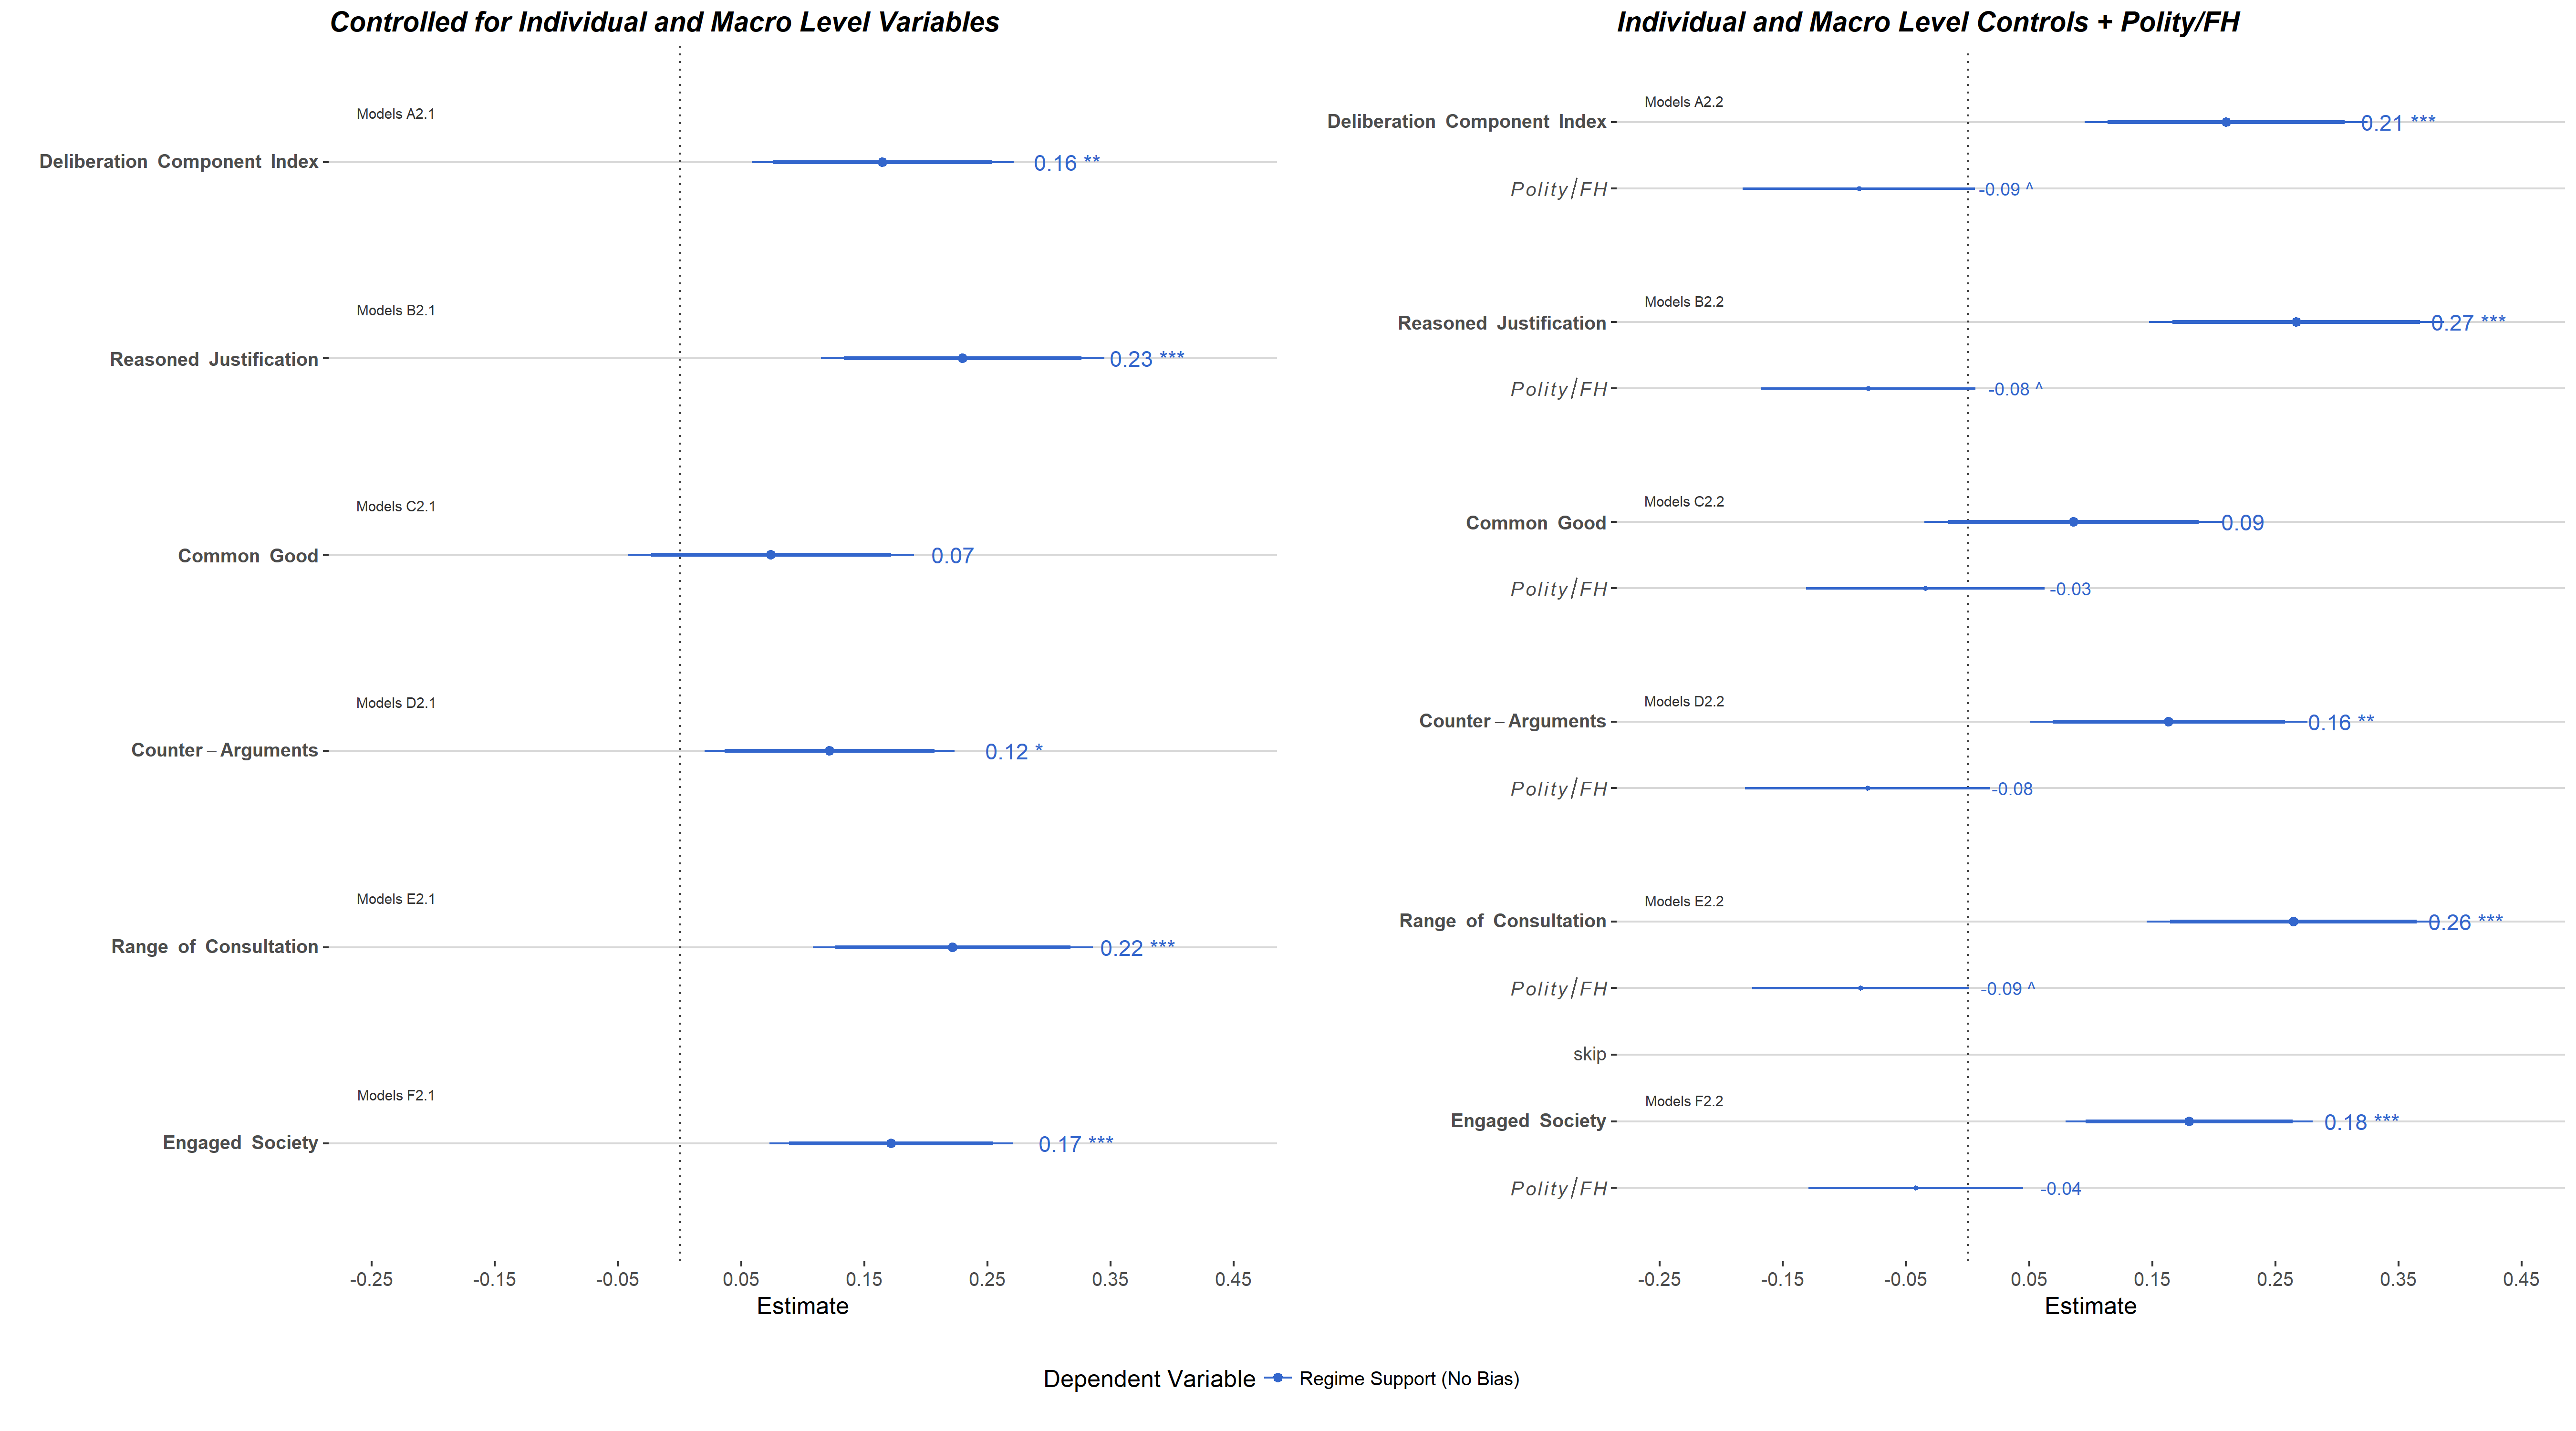
\includegraphics[width=690pt,height=530pt]{images/coefplot_dem.png}
        \flushright
        {\scriptsize $^{***}p<0.001$, $^{**}p<0.01$, $^*p<0.05$, $^{\dagger}p<0.1$. Standardized regression coefficients and 90\% confidence intervals are reported. Reference category for Polity/FH dummies is Anocracy. For the full models see Appendix Table \ref{mod1} and \ref{mod2}. Data weighted to same sample size (=1000). Data Source: see Table \ref{data} in the Appendix. Own calculations  \par}
    \end{figure}
\end{landscape}

After the results for democracies are examined, in the left column of
Figure \ref{reg3}, the effects of the deliberation indicators on regime
support within the non-democracy subsample are reported. Rather similar
to the results for the complete sample, the indicators mostly have weak
negative effects on the unweighted dependent variable.The results follow
no clear pattern for the weighted dependent variables, besides the
previously observed shift towards more positive or less negative
effects. Including the Polity/FH variable in the models has a similar
impact as it had for the democracy subsample and as the dummies had in
the complete sample (see Figure \ref{reg3}, right column): the effects
of the respective deliberation indicators have positive, but small
coefficients in almost all cases (with the exception of Engaged Society,
which is negatively associated for the unweighted regime support).
Weighting regime support has the same impact already observed before
with the dummy variables, by shifting the effects of Polity/FH towards
less negative/more positive coefficients. Recalling the previous
discussion, deliberation indicators with Polity/FH correlations below r
= 0.5 are: Range of Consultation, Reasoned Justification and Common
Good. Overall, no systematic differences can be detected in the results
of the presumably problematic and unproblematic indicators. The same can
be said for the effects of the Polity/FH measure, which has consistently
negative coefficients, which was already observed in the bivariate
correlations as well as the multilevel regression results for the model
including only Polity/FH and the control variables.

\begin{landscape}
    \begin{figure}
        \caption{Non-Demcracy Sample: Models A1.1 to F1.6}
        \label{reg3}
        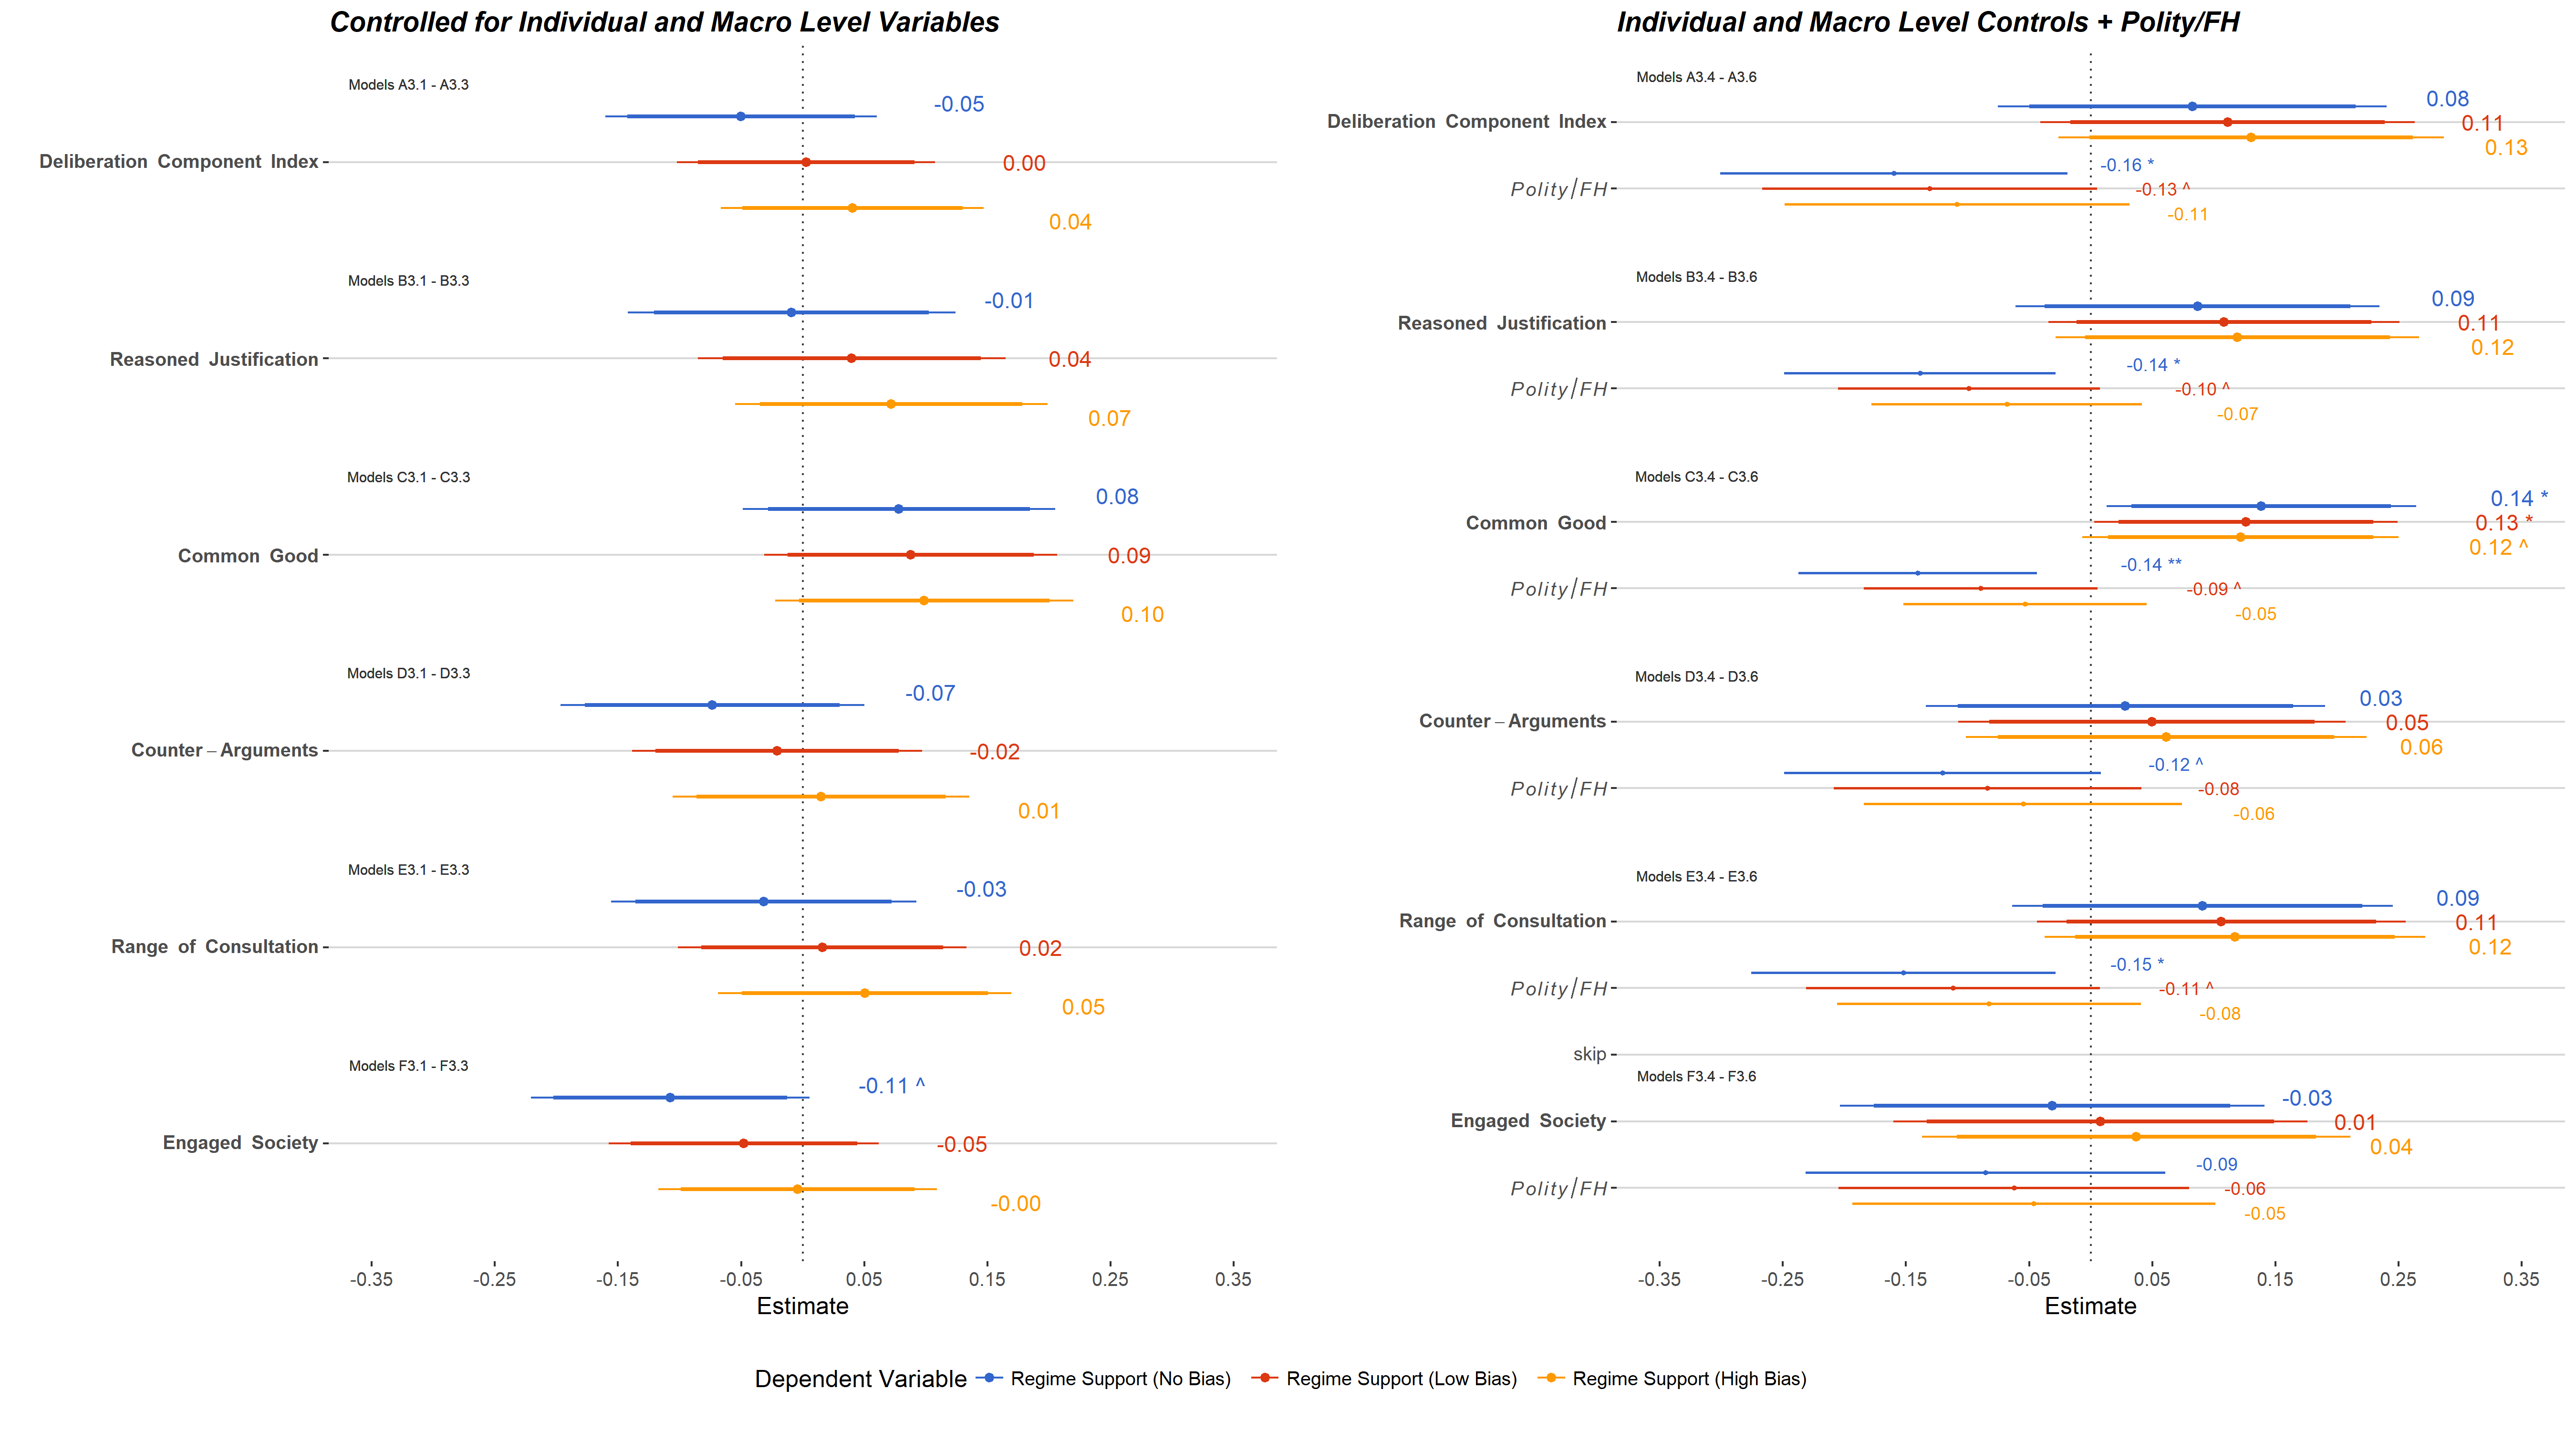
\includegraphics[width=690pt,height=530pt]{images/coefplot_nondem.png}
        \flushright
        {\scriptsize $^{***}p<0.001$, $^{**}p<0.01$, $^*p<0.05$, $^{\dagger}p<0.1$. Standardized regression coefficients and 90\% confidence intervals are reported. Reference category for Polity/FH dummies is Anocracy. For the full models see Appendix Table \ref{mod1} and \ref{mod2}. Data weighted to same sample size (=1000). Data Source: see Table \ref{data} in the Appendix. Own calculations  \par}
    \end{figure}
\end{landscape}

In general, as the theoretical expectation, the empirical evidence for
the effects of deliberation in non-democracies is mixed. Only when
including the Polity/FH variable, the results indicate a weak positive
effect of deliberation, without controlling for the level of democracy,
the effects have negative coefficients. Taking a look at the fit
measurement in Figures \ref{mc5} to \ref{mc7} in the Appendix, one can
see that the models that include Polity/FH as well as the deliberation
components do in general not have a notably higher deviance than the
model including only Polity/FH, indicating that the deliberation
indicators do not contribute to a better model fit for any of the models
(applying all three dependent variables). In regard to the models
including only the deliberation indicators, the models including both
have a better fit, though this only applies for the dependent unweighted
regime support and in no case for the Engaged Society models. In general
it has again to be noted that the non-democracy subsample is affected by
a possible bias in the self-reported regime support and that, as
discussed before, the weighting measure has not been tested for its
accuracy.

In sum, we did find evidence for an effect of deliberation on regime
support, especially and least restricted by limitations within the
democracy subsample. To begin with, general trends can be observed for
the weighting of the dependent variable. In most cases, though not for
the non-democracy subsample, the coefficients of the deliberation
indicators become more positive/less negativen when the weighting is
applied. The effects democracy variables become are less negative for
the weighted dependent variables. A second trend can be observed when
comparing the respective models with and without one of the Polity/FH
measures. In all models, when including Polity/FH, negative effects of
the deliberation indicators become positive and positive effects
increase. This applies to models both presumably problematic and
unproblematic in regard to multicollinearity. The results could indicate
that deliberation has a positive effect on regime support, but at the
same time positively correlates with Polity/FH, which itself has a
negative effect on regime support. This could be interpreted as a
suppressor effect. However, this interpretation has to be done very
cautiously, due to the restrictions of our study.


\end{document}
